\documentclass[sigconf,10pt,review,anonymous]{acmart}

% AI-SEPS 2019
% https://2019.splashcon.org/home/seps-2019#Call-for-Papers
% 10 pages!

%\usepackage{booktabs} % For formal tables

\usepackage{graphicx}
\usepackage{tabularx}
\usepackage{multirow}
\usepackage{mathtools}
\usepackage{amsmath}
\usepackage{xcolor}
\usepackage{colortbl}
\usepackage{amsmath,amssymb,amsfonts}
\usepackage{algorithm}
\usepackage{numprint}
\usepackage{listings}
\usepackage{tabu}
\usepackage{array}

\newcolumntype{P}[1]{>{\centering\arraybackslash}p{#1}}
\newcolumntype{M}[1]{>{\centering\arraybackslash}m{#1}}

% commented out by Roberto: we should stick to the ACM template
%\usepackage{biblatex}

\graphicspath{ {./figures/} }
 
% Copyright
%\setcopyright{none}
%\setcopyright{acmcopyright}
%\setcopyright{acmlicensed}
%\setcopyright{rightsretained}
%\setcopyright{usgov}
%\setcopyright{usgovmixed}
%\setcopyright{cagov}
%\setcopyright{cagovmixed}

% DOI
%\acmDOI{10.475/123_4}

% ISBN
%\acmISBN{123-4567-24-567/08/06}

%Conference
%\acmConference[WOODSTOCK'97]{ACM Woodstock conference}{July 1997}{El Paso, Texas USA}
%\acmYear{1997}
%\copyrightyear{2016}

%\acmArticle{4}
%\acmPrice{15.00}

% These commands are optional
%\acmBooktitle{Transactions of the ACM Woodstock conference}
%\editor{Jennifer B. Sartor}
%\editor{Theo D'Hondt}
%\editor{Wolfgang De Meuter}

% The default list of authors is too long for headers.
\renewcommand{\shortauthors}{A. Maramzin et al.}

\newcommand{\cpp}{C\texttt{++}}

\newcommand{\totalLoops}{1415}
% This percent is computed in data/reduction.ods
\newcommand{\meanReduction}{45}

\lstdefinestyle{mystyle}{
  backgroundcolor=\color{white},   % choose the background color; you must add \usepackage{color} or \usepackage{xcolor}; should come as last argument
  basicstyle=\ttfamily\footnotesize,        % the size of the fonts that are used for the code
  breakatwhitespace=false,         % sets if automatic breaks should only happen at whitespace
  breaklines=true,                 % sets automatic line breaking
  captionpos=b,                    % sets the caption-position to bottom
  commentstyle=\itshape\color{green},    % comment style
  deletekeywords={...},            % if you want to delete keywords from the given language
  escapeinside={\%*}{*)},          % if you want to add LaTeX within your code
  extendedchars=true,              % lets you use non-ASCII characters; for 8-bits encodings only, does not work with UTF-8
  firstnumber=1000,                % start line enumeration with line 1000
  % frame=single,	                   % adds a frame around the code
  keepspaces=true,                 % keeps spaces in text, useful for keeping indentation of code (possibly needs columns=flexible)
  keywordstyle=\color{blue},       % keyword style
  language=C,                 % the language of the code
  morekeywords={*,...},            % if you want to add more keywords to the set
  numbers=none,                    % where to put the line-numbers; possible values are (none, left, right)
  numbersep=5pt,                   % how far the line-numbers are from the code
  numberstyle=\tiny\color{grey}, % the style that is used for the line-numbers
  rulecolor=\color{black},         % if not set, the frame-color may be changed on line-breaks within not-black text (e.g. comments (green here))
  showspaces=false,                % show spaces everywhere adding particular underscores; it overrides 'showstringspaces'
  showstringspaces=false,          % underline spaces within strings only
  showtabs=false,                  % show tabs within strings adding particular underscores
  stepnumber=2,                    % the step between two line-numbers. If it's 1, each line will be numbered
  stringstyle=\color{purple},      % string literal style
  tabsize=2,	                   % sets default tabsize to 2 spaces
  title=\lstname                   % show the filename of files included with \lstinputlisting; also try caption instead of title
}

\lstset{style=mystyle}

%\bibliographystyle{ACM-Reference-Format}
%\addbibresource{main.bib}

\begin{document}

\title{``It Looks Like You're Writing a Loop'': A Learning Parallelisation Assistant}

\author{Aleksandr Maramzin, Christos Vasiladiotis, Roberto Casta\~neda Lozano, Murray Cole, Bj\"orn Franke}
\affiliation{%
  \institution{The University of Edinburgh}
  \streetaddress{Informatics Forum, 10 Crichton Street}
  \city{Edinburgh}
  \state{Scotland}
  \postcode{EH8 9AB}
}
\email{(s1736883,s1576261)@sms.ed.ac.uk, (roberto.castaneda, mic, bfranke)@ed.ac.uk}

%
% The code below is generated by the tool at http://dl.acm.org/ccs.cfm.
% Please copy and paste the code instead of the example below.
%
%\begin{CCSXML}
%<ccs2012>
% <concept>
%  <concept_id>10010520.10010553.10010562</concept_id>
%  <concept_desc>Computer systems organization~Embedded systems</concept_desc>
%  <concept_significance>500</concept_significance>
% </concept>
% <concept>
%  <concept_id>10010520.10010575.10010755</concept_id>
%  <concept_desc>Computer systems %organization~Redundancy</concept_desc>
%  <concept_significance>300</concept_significance>
% </concept>
% <concept>
%  <concept_id>10010520.10010553.10010554</concept_id>
%  <concept_desc>Computer systems organization~Robotics</concept_desc>
%  <concept_significance>100</concept_significance>
% </concept>
% <concept>
%  <concept_id>10003033.10003083.10003095</concept_id>
%  <concept_desc>Networks~Network reliability</concept_desc>
%  <concept_significance>100</concept_significance>
% </concept>
%</ccs2012>
%\end{CCSXML}

%\ccsdesc[500]{Computer systems organization~Embedded systems}
%\ccsdesc[300]{Computer systems organization~Redundancy}
%\ccsdesc{Computer systems organization~Robotics}
%\ccsdesc[100]{Networks~Network reliability}

\begin{abstract}
% what is the problem
  Despite decades of intensive research, software parallelisation remains a
  challenging task that usually requires a significant degree of manual effort.
%
  Typically, this task involves identifying the loops that consume most of the
  execution time in a program, analysing whether they are parallelisable, and if
  so, transforming them into a parallel form.
%
  Among these steps, parallelisability analysis is particularly time consuming
  and often requires a high level of expertise.

% what is our solution
  This paper introduces an assistant that reduces the manual parallelisation
  effort by providing the programmer with a ranking of the loops based on their
  execution time and, crucially, their parallelisability likelihood.
%
  Parallelisability is predicted using a novel machine-learning model based on
  static loop features such as iteration and dependence analysis results.
%
  The model is trained, validated, and tested on~\numprint{\totalLoops{}}
  labelled loops.
%
  Despite the limited size of the data set, it achieves a prediction accuracy
  higher than~90\%.

% why does it matter
  Experiments on the SNU NAS Parallel Benchmarks show that, on average,
  following the assistant's ranking reduces by~\meanReduction{}\% the number of
  loops that need to be analysed manually to achieve expert-level speedup.
% what follows from it
  Given the high level of expertise involved in manual parallelisation, such a
  reduction can translate into substantial development cost savings and ease the
  much-needed transition of legacy code bases to parallel computing.

%% \quad Since automatically parallelizing compilers have failed to deliver significant performance improvements, programmers are still forced to parallelize legacy software manually for all but some niche domains. Rather than hoping for an elegant silver bullet, we acknowledge the role of a human expert in the parallelization process and develop a \textit{smart} parallelization assistant.\newline\null
%% \quad In its essence our assistant is yet another application of machine learning techniques to the field of optimizing compilers, which tries to predict the parallelisability property of program loops.
%% We use a version of NAS Parallel Benchmarks (NPB) hand-annotated with OpenMP parallelisation pragmas to train our model. We show that it is possible to achieve a good prediction accuracy of around 90\% for our problem using only static program features. We outperform all available baseline random predictors working at an accuracy ranging between 40\% and 70\%. To get a real practical application of our techniques, we integrate our trained ML model into 2 assistant schemes. Our schemes mitigate the effects of ineradicable statistical errors and make them not that critical. As a result we extend capabilities of Intel \cpp{} compiler in the task of parallelism discovery and increase the amount of parallelism found in SNU NPB benchmarks from 81\% to 96\%. The second scheme is basically an assistant, which directs programmer efforts by pointing the loops, which are the most highly likely to be parallelisible and profitable as well. Thus, decreasing the efforts and time it takes to parallelize a program manually.

%
%Parallelising compilers comprise powerful program analyses, yet they fail to deliver a parallel speedup on real-world programs outside the domain of Fortran-style array based computations due to the limits of static dependence and profitability analyses. Decades of intensive research have not yet delivered a breakthrough, and we do not expect a major breakthrough in static analysis in the near future. In order to accelerate a software a programmer still has to manually analyse and parallelise it. At the same time, the field of machine learning (ML) has made a massive progress and ML techniques are, in fact, already used in parallelising compilers to support profitability analysis and scheduling decisions. In this work we apply ML to predict parallelisability property of program loops and to guide a human effort of software parallelisation.\newline\null
%\quad We use a version of NAS Parallel Benchmarks (NPB) annotated with OpenMP parallelisation pragmas to train our model to predict loop parallelisability property. We show that using only static program features we can achieve the average prediction accuracy of around 90\% against various baselines (random, most frequent, etc.) ranging from 40\% to 70\%. Inherent to all statistical methods false positives comprise around 6\% of cases. To eliminate the danger of false positives we require a final programmer approval and propose 2 schemes of providing a programmer with a parallelisation feedback. The first scheme enhances Intel \cpp{} Compiler (ICC) parallelism discovery in SNU NAS benchmarks from 81\% to 96\% of all SNU NPB parallel loops. The second takes benchmark profiles and provides a programmer with a loop rankings to follow in benchmark parallelisation. Enhanced ranking allows a programmer to converge to the best achievable performance on a benchmark faster, than by following a mere profile based order.
%Here: Novel use of ML in parallelisation to guide human effort: Once all
%automatically parallelisable loops have been parallelised using state-of-the-art
%auto-parallelisers, ML predicts which loops to parallelise next. 
%Evaluated and outlook
%In this work we 
%All modern hardware is highly parallel, but in order to fully utilise availability of all these resources software must be parallel as well. There are numerous approaches to the task of software parallelisation ranging from manual approaches to fully automatic ones. In this work we investigate a relatively new approach to the task of software parallelisation: a machine learning assisted one. We use a version of NAS Parallel Benchmarks annotated with OpenMP parallelisation pragmas to train our model to predict loop parallelisability. We achieve 93\% generalised prediction accuracy with a baseline (random predictor) around 60\%. We study parallelisability of NAS benchmarks and its utilisation with Intel \cpp{} Compiler (ICC) and propose a scheme, which might be used to supplement ICC with a ML-based tool. Proposed scheme increases ICC parallelisation coverage in the NAS Parallel Benchmarks from 86\% to 99\% and comes close to its algorithmic limit. After that we show, that for majority of NAS benchmarks this parallelisation coverage increase transforms into the actual performance improvements as well. We achieve an average speedup of 2.5x relative to the state-of-the-art parallelising Intel \cpp{} compiler and come closer to 3.5x average speedup of the expert hand-parallelised version.

\end{abstract}

%
% Keywords. The author(s) should pick words that accurately describe the work being
% presented. Separate the keywords with commas.
%\keywords{datasets, neural networks, gaze detection, text tagging}

\maketitle

\section{Introduction}

% problem: the need for manual parallelisation, auto-parallelisation does not deliver desired performance improvements

Parallel hardware is ubiquitous through the entire spectrum of computing
systems, from low-end embedded devices to high-end supercomputers.
%
Yet, most of the existing software is written in a sequential fashion.
%
Despite decades of intensive research in automatic software
parallelisation~\cite{TODO}, fully exploiting the potential of modern hardware
still requires a significant manual effort.
%
Given the difficulty of the obstacles faced by automatic parallelisation today,
we do not expect that programmers will be liberated from performing manual
parallelisation in the near future~\cite{TODO}.

% solution: parallelisation assistant

This paper introduces a parallelisation assistant that aids the programmer in
the process of parallelising a program in the frequent case where automatic
approaches fail to do so.
%
The assistant reduces the manual effort in this process by presenting the
programmer a ranking of the program loops that are most likely to 1) be
parallelisable and 2) improve the program's performance by being parallelised.
%
Thus, it improves the traditional, profile-guided process by also taking into
account how likely it is that each of the profiled loops can be parallelised.

% how?

At the core of the assistant is a novel machine-learning (ML) model of loop
parallelisability.
%
Loops are a compelling candidate for parallelisation, as they are naturally
decomposable and tend to capture most of the execution time in a program.
%
Furthermore, focusing on loops allows the model to leverage a large amount of
specific analyses available in modern compilers, such as generalised iterator
recognition~\cite{TODO} and loop dependence analysis~\cite{TODO}.
%
The model encodes the result of these analyses together with basic properties of
the loops as features.

The loop parallelisability model is trained, validated, and tested
on~\numprint{\totalLoops{}}~loops from the SNU NAS Parallel
Benchmarks~\cite{TODO}.
%
The loops are labelled using a combination of expert OpenMP~\cite{TODO}
annotations and optimisation reports from Intel \cpp{} Compiler (ICC), a
state-of-the-art parallelising compiler~\cite{TODO}.
%
The model is evaluated on multiple state-of-the-art machine learning algorithms,
including tree-based methods, support vector machines, and neural networks.
%
The evaluation shows that, despite the limited size of the data set, using
support vector machines allows the model to achieve a prediction accuracy higher
than 90\%.
%
% Note: the "detected parallelism increase" is 945/995 - 812/995 = 0.1336683417.
%
The model increases the amount of parallelism detected by ICC by~13\% while
introducing a false positive rate (misclassifying non-parallelisable loops)
of~7\%. \textcolor{red}{(FIXME: taken from~Figure~\ref{fig:accuracy},
  double-check these numbers)}

% TODO: mention that we use standard techniques for feature extraction,
% hyper-parameter tuning, and cross-validation?

The parallelisation assistant combines inference on the parallelisability model
with traditional profiling to suggest loops with high likelihood of being
parallelisable and impacting the program's performance.
%
An evaluation on seven programs from the SNU NAS Parallel Benchmarks shows that
the programs' performance tends to improve faster as loops are parallelised in
the order suggested by the assistant compared to a traditional ordering based on
profiling.
%
On average, following the order suggested by the assistant reduces
by~\meanReduction{}\% the number of loops that need to be analysed manually to
achieve expert-level speedup.
%
Given the high level of expertise involved in manual analysis, such a reduction
can translate into substantial development cost savings.

%% \quad There is a number of well-known problems in the field of parallel software engineering, which compose the ground our work grows on. Parallel hardware is omnipresent in the whole spectrum of computers from low end devices up to the high end supercomputers. Yet, in order to utilise all these available hardware capabilities the software has to be parallel as well. Unfortunately, the legacy software is written in a sequential fashion and in order to make it run faster we either have to parallelise it manually or rely on automatic parallelisation techniques. Both approaches have their pros and cons. The former require parallel programming expertise on top of the application domain knowledge, the latter is limited to the narrow niche of scientific FORTRAN-like codes. Decades of intensive research have not yet delivered a breakthrough, and we do not expect a major breakthrough in automatic parallelisation in the near future. In order to accelerate a software a programmer still has to manually analyse and parallelise it. Indeed, as our experiments show (see section [?]), even the state-of-the-art Intel \cpp{} compiler cannot achieve significant performance improvements on highly parallel by their nature NAS Parallel Benchmarks (NPB). Meanwhile, the field of machine learning (ML) has made a massive progress and continuously finds itself to be effective and practical in a growing set of application areas. ML based techniques are not new to the field of optimising compilers either. As survey [?] shows ML techniques have been applied to tasks ranging from the selection of the best compiler flags to choosing the most optimal mapping of parallelism onto heterogeneous hardware resources.\newline\null
%% \quad In our work we acknowledge the role of a human programmer in the software parallelisation process and develop a supplementary assistant guiding the human efforts by highlighting program loops, which are highly likely to be parallelisable and profitable as well. Our tool targets the phase of parallelism discovery 


%% For several decades, parallelising compilers have been the subject of intensive academic research \cite{XXX} and industrial investment \cite{XXX}. Yet, for most real-world applications they fail to deliver parallel performance \cite{XXX}.


%% In this paper we take a different approach: We acknowledge the role of the human expert in the parallelisation process, and develop a machine learning based assistant guiding the users to focus their resources on those loops most likely to result in a positive return-of-investment (ROI). We do not aim to completely automate parallelisation including program analysis and transformation, but instead assist the user by suggesting an ordered ranking of loops for manual parallelisation, where this ordering considers both the estimated effort and profit of parallelising each loop in turn.

\paragraph{Motivating example}

As a motivating example, let us consider the CG program from the SNU NAS
Parallel Benchmarks.
%
Table~\ref{tab:ranking} shows the top three CG loops as ranked by the Intel
Profiler (purely based on their execution time) and by the parallelisation
assistant (additionally taking into account predicted parallelisability).
%
Both rankings include the same loops, but, crucially, the loops are ranked
in a different order.
%
Among the three loops, only \texttt{cg.c:509} (marked in bold in the table) is
parallelisable, while the other two loops (\texttt{cg.c:326} and
\texttt{cg.c:484}) are not.

\begin{table}
  \caption{Ranking of the top three CG loops.}
  \label{tab:ranking}
  \begin{minipage}{\columnwidth}
  \begin{center}
    \begin{tabu}{ccccc}
      \hline
      \rowfont{\bfseries}
      \multicolumn{2}{c}{profiler} & \multicolumn{3}{c}{assistant} \\\hline
      \rowfont{\bfseries}
      loop & ranking & loop & ranking & parallel \\\hline
      \texttt{cg.c:326} & 0.93 & \textbf{\texttt{cg.c:509}} & \textbf{0.34} & 85\%\\
      \texttt{cg.c:484} & 0.91 & \texttt{cg.c:326} & 0.17 & 29\%\\
      \textbf{\texttt{cg.c:509}} & \textbf{0.89} & \texttt{cg.c:484} & 0.05 & 8\%\\
    \end{tabu}
  \end{center}
  \end{minipage}
\end{table}%

Following the profiler ranking as in traditional profile-guided parallelisation
(two first columns in Table~\ref{tab:ranking}), the loops \texttt{cg.c:326} and
\texttt{cg.c:484} are selected first for manual analysis.
%
The analysis determines that these loops are not parallelisable, due to
inter-iteration dependencies and side effects caused by system calls (see
Listing~\ref{lst:main_iter}).
%
Finally, manual analysis of loop \texttt{cg.c:509} (see
Listing~\ref{lst:reduction}) recognises that it computes an array of reductions
and is thus parallelisable.
%
Just parallelising this loop speeds up CG by a factor of 2.8, which is 80\% of
the speedup obtained by an expert parallelisation of the entire program.

In contrast to the profiler, this paper's assistant (two last columns in
Table~\ref{tab:ranking}) predicts that loop \texttt{cg.c:509} is parallelisable
(likelihood of 85\%) while loops \texttt{cg.c:326} and \texttt{cg.c:484} are not
(likelihood of just 29\% and 8\%).
%
Consequently, it ranks the loop \texttt{cg.c:509} at the top, allowing the user to
achieve the same program speedup without having to analyse loops
\texttt{cg.c:326} and \texttt{cg.c:484}.
%
% Note: the 100 lines of code are counted using 'cloc code/cg-326.c'.
%
The manual effort savings are significant, considering that \texttt{cg.c:326} is
an outermost loop consisting of 100 lines of code (including its called function
\texttt{conj\_grad} where \texttt{cg.c:484} and \texttt{cg.c:509} are defined)
whereas \texttt{cg.c:509} is a tiny loop consisting of just the six lines shown
in Listing~\ref{lst:reduction}.

\begin{lstlisting}[caption={\texttt{cg.c:326}. Longest running loop in CG. The loop cannot be parallelised due to
inter-iteration dependences and side effects caused by system calls.},label={lst:main_iter},language=C]
for (it = 1; it <= NITER; it++) {
  ...
  if (timeron) timer_start(T_conj_grad);
  conj_grad(colidx,rowstr,x,z,a,p,q,r,&rnorm);
  if (timeron) timer_stop(T_conj_grad);
  ...
  printf("    %5d       %20.14E%20.13f\n", it, rnorm, zeta);
  ...
}
\end{lstlisting}

\begin{lstlisting}[caption={\texttt{cg.c:509}. Longest running loop in CG \emph{that can be parallelised}.},label={lst:reduction},language=C]
for (j = 0; j < lastrow-firstrow+1; j++) {
  suml = 0.0;
  for (k = rowstr[j]; k < rowstr[j+1]; k++)
    suml = suml + a[k]*p[colidx[k]];
  q[j] = suml;
}
\end{lstlisting}

\paragraph{Contributions}

In summary, this paper makes the following contributions:
%
\begin{itemize}
\renewcommand\labelitemi{$\vartriangleright$}
\renewcommand\labelitemii{$\bullet$}
\item Designed an ML based model of loop parallelisability quantifying the latter (Section~\ref{predicting_parallel_loops}) and ranking program loops
    \begin{itemize}
    \item Devised loop parallelisability metrics (ML loop features)
    \item Prepared a labelled training set with classification labels
    derived from SNU NPB OpenMP \textit{\#pragmas} as well as Intel Compiler optimisation reports
    \item Set and tuned an ML train/test methodology
    \end{itemize}
\item Conducted a thorough evaluation of the model demonstrating prediction accuracy
  higher than 90\% on~\numprint{\totalLoops{}}~loops from the SNU NAS Parallel
  Benchmarks (\textcolor{red}{Section~4})
\item Integrated the model into a parallelisation assistant scheme that automatically ranks promising loops by combining profiling information and model inference (\textcolor{red}{Section~5})
    \begin{itemize}
    \item Demonstrated improved parallelism discovery capabilities of assistant in comparison with Intel Compiler 
    \end{itemize}
\item Deployment of the assistant on SNU NAS Parallel Benchmarks demonstrating its potential to ease parallelisation process and converge to the maximum attainable performance faster
    \begin{itemize}
    \item Conducted a performance study of SNU NPB with the state-of-the-art Intel Compiler
    \item Parallelisied SNU NPB following profiler and assistant suggested loop orders and plotted performance convergense curves
    \end{itemize}

a demonstration of the assistant's potential to reduce the manual effort
  involved in the traditional profile-guided parallelisation methodology
  (\textcolor{red}{Section~6}).
\end{itemize}
%% 1) We show that it is possible to learn loop
%% have successfully learnt the parallelisability property o
%% 2) We conduct a study of Intel Compiler's behaviour on SNU NPB benchmarks. We summarise the exact optimizations applied (see section [?]), classify missed parallelisation opportunities (see section [?]) and
%% \subsection{Overview}

%% \subsection{Paper structure}
%% \quad The most substantial part of this work was aimed at the creation of machine learning (ML) based model, capable of accurate prediction of loop parallelisability property. Section \ref{predicting_parallel_loops} describes all the details of machine learning part including the features we chose and the exact training/testing methodology we used. But even close to perfect prediction accuracy is not enough, if we cannot find a real practical application to utilise our predictor. Section \ref{practical_applications} proposes 2 complementary schemes we might integrate our predictor into. The first scheme helps Intel ICC compiler to discover additional parallelism. The second scheme is basically software manual parallelisation assistant working with a program profile and directing human efforts at the most likely to be parallelisible (and profitable as well) loops. Section \ref{evaluation} presents a quantitative report on our work.  


\section{Background}

\subsection{Parallelism Discovery}

\subsection{Profitability Analysis}

For example, SUIF \cite{Wilson:1994:SIR:193209.193217} uses a simple heuristic based on the product of statements per loop iteration and number of loop iterations to decide whether a parallelizable loop should be scheduled to be executed in parallel. In contrast, \cite{Tournavitis:2009:THA:1542476.1542496} uses a machine learning based heuristic, which consumes \textit{dynamic} program features collected in a separate profiling stage, to decide if and how a potentially parallel loop should be scheduled across multiple processors.

\section{Predicting Parallel Loops}
\label{predicting_parallel_loops}
\quad This section describes the exact way we applied supervised machine learning (ML) techniques to the problem of loop parallelisability prediction. Here we describe the features we choose to represent program loops and the way we collect our data, as well as the whole ML train/test \textit{methodology}. The methodology consists of a number of stages arranged in a \textit{pipeline} (data extraction, data preprocessing, automatic feature selection, ML model selection and the search of its hyper-parameter spaces, training/validation/testing, etc.). All technical background on ML can be found in the book \cite{James:2014:ISL:2517747}.\newline\null
\quad In order to achieve the best ML performance our features and the exact parameters of methodology have been iteratively tuned and refined with the help of K-fold CV. Predictive \textit{accuracy}, \textit{recall} and \textit{precision} scores were used as selection criteria. To get the most accurate and honest assessment of our ML models we kept the testing data hidden and used only the training data during all ML pipeline stages. Following subsections present the final results rather than the path towards them.
\subsection{Overview}
\label{ml_overview}
\quad The machine learning (ML) task we solve in our project can be presented as \textbf{supervised ML classification problem}: \textit{create an ML based model of loop parallelisability and train it to classify loops of Seoul National University implementation \cite{snu-npb-benchmarks} of NAS Parallel Benchmarks \cite{nasa-parallel-benchmarks} as parallelizable or not.}\newline\null 
\quad We used facilities of \textit{scikit-learn} \cite{scikit-learn} Python library for all ML related tasks. To conduct various ML training/testing experiments in the search of the best ML model faster and easier we developed a Python scripting framework based on the scikit-learn library taking an input data (train and test) along with an ML pipeline INI configuration file. Configuration file allows us for a flexible change in the settings of an experiment (ML model to use, its hyper-parameter search space, the exact automatic feature selection methods, etc.). The following sections give a detailed description of all ML pipeline stages.
\subsection{Loop Analysis \& Features}
\label{loop_analysis_and_features}
\begin{comment}
\quad We base our feature engineering efforts on the vast body of work done in the field of optimising compilers. Particularly in the domain of program dependence analysis \cite{Kennedy:2001:OCM:502981}. 
We dump PDGs in a dot format and systematically use these visualisations in our work in order to debug and decide on the best features to use.
\end{comment}
\quad One of the most important parts in applying ML techniques to a given problem is the \textit{feature engineering} task. In our project we need to pick the right program loop features, which are the most reflective of loop parallelizability property. In the task of coming up with a set of loop features we are guided by general program dependence analysis theory \cite{Kennedy:2001:OCM:502981}, the exact types of loops present in SNU NPB benchmarks and Intel \cpp{} compiler optimization reports.\newline\null
\quad There is a range of SNU NPB loops, which escape Intel compiler parallelization for different reasons: indirect array references, unrecognised reductions on arrays, pointers with statically unknown memory locations, etc. But all that range of reasons is going to ultimately materialise into data and control dependencies present between loop instructions, represented as edges on the Program Dependence Graph (PDG) \cite{Ferrante:1987:PDG:24039.24041} of a loop. Figure \ref{fig:pdg} shows an example of a PDG built for a simple loop and visualised with our tool.\newline\null
\begin{figure}[h]
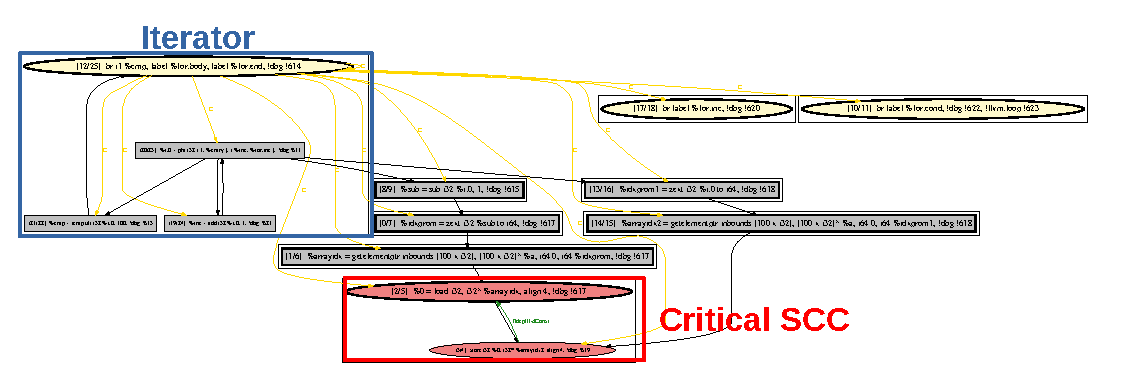
\includegraphics[width=0.5\textwidth]{figures/pdg_example.pdf}
\caption{Example of PDG of a simple loop with a cross-iteration dependency built and visualised by our tool. These graph visualisations were used during tool debugging and feature engineering processes.}
\label{fig:pdg}
\end{figure}
\quad The PDG graph consists of LLVM IR instructions as nodes and different sorts of dependencies between them as graph edges. Dependence relation lies at the the very essence of loop parallelization, on the other hand just counting the number of dependence edges in the PDG of a loop is not enough to make decisions about loop parallelizability. Dependence relations might exist only withing one loop iteration or span across multiple, thus preventing parallelization.\newline\null
\quad To refine our features we use the work on \textit{generalised loop iterator recognition} \cite{Manilov:2018:GPI:3178372.3179511}. Generalised iterator recognition analysis separates \textit{loop iterator} from the actual \textit{loop payload} providing us with finer loop partitions to base our features on. As work \cite{Manilov:2018:GPI:3178372.3179511} explains, loop iterator is a \textit{strongly connected component (SCC)} on the PDG with no incoming dependence edges. There are SCCs in the payload as well. Usually they consist of just 1 instruction, but when we have a cross-iteration dependency they tend to grow larger and form a cycle. We call such SCCs \textit{critical}, as ones preventing parallelization. Figure \ref{fig:pdg} highlights both the iterator and the critical SCC present in the example loop. Inner loop iterators tend to appear as critical SCCs for the outer loop as well. To separate these cases we use \textit{inner loops number} and \textit{loop depth} as separate ML features.\newline\null  
\quad The feature engineering process has been conducted iteratively and has been guided by the change in ML models predictive performance with the addition of one feature or the other. This process involved several methods. First, we tried to capture in our features the differences between PDG visualizations for parallel and non-parallel loops. Then we studied the source code of SNU NPB benchmarks along with ICC optimization reports and tried to understand why ICC failed to parallelize some of SNU NPB loops and transfer those insights into reflective features.\newline\null
\quad We ended up with a set of 74 static loop features, which are based on the structural properties of PDG and the types of instructions constituting them. Table \ref{tab:loop_features} summarizes the main groups of devised features.\newline\null
\quad Many of our features have a simple and intuitive motivations behind them. Loop proportion related features are backed up by the the fact, that bigger loops are harder to parallelize. Big iterators contain complex cross-iteration transitions (e.g linked-list update), unknown iteration numbers, etc. Critical SCCs limit loop parallelization further. Cohesion features do not have an apparent intuition. They characterise how tightly components of loops are coupled together in terms of the number of edges between them. Loop dependencies number features count the number of edges in different loop parts as well as their types. Loop instructions nature characterise the types of loop instructions, assigning more importance to memory reads/writes, calls, branches. Uninlined funtion calls usually prevent loop parallelization. Intensive memory work (memory read/write fraction features) complicates parallelization as well.   
\begin{comment}
\begin{table*}[h!]
    \centering
    \begin{tabular}[c]{|p{2.5cm}|p{4.0cm}|p{9.0cm}|}
        \hline
        feature groups & features & description\\
        \hline
        \multirow{3}{2.5cm}{Loop Proportions} & Absolute Size & the number of LLVM IR instructions\\\cline{2-3}
        & Payload Fraction & $\frac{payload instructions number}{whole loop instructions number}$\\\cline{2-3}
        & Proper SCCs Number & number of payload SCCs with more than 1 instruction\\\cline{2-3}
        \hline
        Loop Dependencies & \multicolumn{2}{|p{13.0cm}|}{The number of PDG edges corresponding to different dependence classes: read/write order (\textbf{True}, \textbf{Anti}, \textbf{Output}), dependency media (\textbf{Register}, \textbf{Memory}, \textbf{Control}), other (\textbf{Confused}, \textbf{Cross-Iteration})} \\
        \hline
        \multirow{2}{2.5cm}{Loop Cohesion} & Iterator/Payload & $\frac{Num of Edges Between Iterator/Payload}{Total Loop Edges Num}$\\\cline{2-3}
        & Critical/Regular Payload & $\frac{Num of Edges Between Critical/Regular Payload}{Total Loop Payload Edges Num}$\\
        \hline
        Loop Nature & \multicolumn{2}{|p{13.0cm}|}{The number of different kinds of critical to loop parallelisability instructions (memory reads/writes, calls, branches, etc.). These numbers are computed for different loop parts (iterator, payload, critical payload)} \\
        \hline
    \end{tabular}
    \caption{The set of static code features devised to capture loop parallelisability property.}
    \label{tab:loop_features}
\end{table*}
\end{comment}
\begin{table*}[!h]
  \begin{minipage}{\linewidth}
  \begin{center}
    \begin{tabu}{M{3cm}M{5cm}M{8cm}}
      \hline
      \rowfont{\bfseries}
      Feature groups & Features & Description\\\hline
      \multirow{3}{*}{Loop Proportions} & Absolute Size & the number of LLVM IR instructions\\%\hline
      & Payload Fraction & $\frac{payload instructions number}{whole loop instructions number}$\\%\hline
      & Proper SCCs Number & number of payload SCCs with more than 1 instruction\\\hline
      Loop Dependencies & \multicolumn{2}{M{13cm}}{The number of PDG edges corresponding to different dependence classes: read/write order (\textbf{True}, \textbf{Anti}, \textbf{Output}), dependency media (\textbf{Register}, \textbf{Memory}, \textbf{Control}), other (\textbf{Confused}, \textbf{Cross-Iteration})}\\\hline
      \multirow{2}{*}{Loop Cohesion} & Iterator/Payload & $\frac{Num of Edges Between Iterator/Payload}{Total Loop Edges Num}$\\
        & Critical/Regular Payload & $\frac{Num of Edges Between Critical/Regular Payload}{Total Loop Payload Edges Num}$\\
        \hline
      \end{tabu}
  \end{center}
  \end{minipage}
  \caption{The set of static code features devised to capture loop parallelisability property.}
  \label{tab:loop_features}
\end{table*}%
\subsection{Feature Extraction}
\label{feature_extraction}
\quad To extract all devised loop features from SNU NPB benchmarks we developed \textbf{PParMetrics (Pervasive Parallelism Metrics)} tool, based on the LLVM compiler infrastructure \cite{llvm-compiler-infrastructure}\cite{Lattner:2004:LCF:977395.977673}. The tool is basically a set of LLVM function passes working on the SSA-based LLVM IR and can be found on the GitHub \cite{github-ppar-tool}.\newline\null
\quad The tool works by building data, memory and control dependence graphs (DDG, MDG, CDG) and combining them into the final program dependence graph (PDG) \cite{Ferrante:1987:PDG:24039.24041} for all loops found in program functions. For these purposes the tool uses standard \textit{def-use chains}, \textit{post-dominator trees} and \textit{dependence analysis} passes available in the LLVM. Once all graphs are built we run the search of strongly-connected components (SCCs) on them and recognise loop iterators. The final step is to traverse all these graphs computing devised metrics (ML features) and dump all that information into the file to be later fed into scikit-learn based ML scripts.
\subsection{Feature Selection}
\label{feature_selection}
\quad The feature engineering task resulted into a quantitative description of program loops being characterised by feature vectors of length 74. Many features in the set are just slightly different variations on the same property and can potentially result into ML model over-fitting. To avoid that we need to discard some irrelevant or redundant features based on empirical data in an automated fashion. Doing so also aligns our methodology with a standard accepted one.\newline\null   
\quad Our ML pipeline scripts can be configured to apply an arbitrary sequence of different scikit-learn feature selection methods. First we filter out all features with a low variance score, then we fit a decision tree based model and select all features with importance score above the threshold. Then we repeatedly run recursive feature elimination by the cross-validation (RFECV) in an attempt to improve several targets: recall, precision and accuracy scores. Table \ref{tab:best_features} illustrates the relative ranking of the 10 highest scoring features in our automatic feature selection runs.\newline\null  
\quad SNU NPB benchmarks contain a lot of uninlined function calls and it is unsurprising that the amount of call instructions in the payload of a loop ranks the highest. Despite the absence of straightforward intuition behind cohesion metrics, they tend to correlate with parallelisation labels well. Loops heavy on memory writes also significantly affect the parallelisability property.
\begin{comment}
\begin{table}[h!]
    \centering
    \begin{tabular}[c]{|p{5.5cm}|p{1.5cm}|}
        \hline
        feature & importance\\
        \hline
        payload call fraction & 23.5\\
        \hline
        payload mem dep num & 4.0\\
        \hline
        iter/payload non-cf cohesion & 18.5\\
        \hline
        iter/payload total cohesion & 3.2\\
        \hline
        payload mem write fraction & 6.1\\
        \hline
        critical payload non-cf cohesion & 2.9\\
        \hline
        loop absolute size & 5.7\\
        \hline
        payload getelemptr fraction & 2.7\\
        \hline
        critical payload getelemptr count & 5.3\\ 
        \hline
        critical payload total cohesion & 2.6\\
        \hline
    \end{tabular}
    \caption{Relative importance of our features, ranked by fitting tree based ML model.}
    \label{tab:best_features}
\end{table}
\end{comment}
\begin{table}
  \begin{minipage}{\columnwidth}
  \begin{center}
    \begin{tabu}{ll}
      \hline
      \rowfont{\bfseries}
      \multicolumn{1}{l}{Feature} & \multicolumn{1}{l}{Importance}\\\hline
      payload call fraction & 23.5\\
      iter/payload non-cf cohesion & 18.5\\
      payload mem write fraction & 6.1\\
      loop absolute size & 5.7\\
      critical payload getelemptr count & 5.3\\
      payload mem dep num & 4.0\\
      critical payload non-cf cohesion & 2.9\\
      payload getelemptr fraction & 2.7\\
      critical payload total cohesion & 2.6\\\hline
      \end{tabu}
  \end{center}
  \end{minipage}
  \caption{Relative importance of our features, ranked by fitting a tree based ML model.} 
  \label{tab:best_features}
\end{table}%

\subsection{Model Selection}
\label{model_selection}
\quad We use several machine learning algorithms available in the scikit-learn library to compare and find the best one. Among these are tree-based methods like (decision trees (DT), random forests (RFC), boosted decision trees (AdaBoost)), support vector machines (SVC) and neural network based multi-layer perceptron (MLP). Section \ref{evaluation_kfold} shows, that all these models perform comparably good with SVC and MLP being slightly better. 

\subsection{Model Hyper-Parameter Selection}
\label{model_hyper_parameter_selection}
\quad For any chosen parametric machine learning model we need to pick the right set of model hyper-parameters. Hyper-parameters are parameters that are not directly learnt within models. Typical examples include C, kernel and gamma for Support Vector Classifiers (SVC), exact architecture for neural network based models, etc. For any given model we use exhaustive hyper-parameter grid search and pick the node of the grid with the best cross validation score on the training set. Table presents hyper-parameter spaces we search for different models.

\begin{comment}
\begin{table}[h!]
    \centering
    \begin{tabular}[c]{|p{2.0cm}|p{5.0cm}|}
        \hline
        model & hyper-parameter space\\
        \hline
        SVC & \textbf{kernel}: rbf,sigmoid,poly, \textbf{C}: 1,10,$10^2$,$10^3$ \textbf{$\gamma$}: 1,$10^{-1}$,$10^{-2}$,$10^{-3}$,$10^{-4}$\\
        \hline
        DT RFC AdaBoost & \textbf{n\_estimators}: 1,2,5,10,50,100 \textbf{max\_depth}: 1,3,5,7,10,15,20,30,50 \textbf{min\_samples\_split}: 0.05,0.1,0.2,0.5,0.7,0.9 \textbf{min\_samples\_leaf}: 1,5,10,15,30,50,60,70,100 \textbf{max\_features}: 1,5,10,15,30,50,70\\
        \hline
        MLP & \textbf{activation}: logistic,relu,tanh \textbf{solver}: lbfgs,sgd,adam \textbf{hidden\_layes\_sizes}: (5;5),(10),(10;10),(10;5),(5;2),(2;5) \textbf{$\alpha$}: $10^2$,10,1,$10^{-1}$,$10^{-2}$\\
        \hline
    \end{tabular}
    \caption{Hyper-parameter spaces to search for an optimal point for different ML models.}
    \label{tab:hyper_param_space}
\end{table}

\begin{table}
  \begin{minipage}{\columnwidth}
  \begin{center}
    \begin{tabu}{ccc}
      \hline
      \rowfont{\bfseries}
      \multicolumn{1}{c}{Model} & \multicolumn{2}{c}{Hyper-Parameter Space}\\\hline
      \multirow{3}{*}{\textbf{SVC}} & \textit{kernel:} & rbf, sigmoid, poly\\%\hline
      & \textit{C:} & 1, 10, $10^2$, $10^3$\\
      & \textit{$\gamma$:} & 1, $10^{-1}$, $10^{-2}$, $10^{-3}$, $10^{-4}$\\\hline
      \multirow{5}{*}{\textbf{\shortstack[c]{DT\\AdaBoost\\RFC}}} & \textit{n\_estimators:} & 1, 2, 5, 10, 50, 100\\%\hline
      & \textit{max\_depth:} & 1, 3, 5, 7, 10, 15, 20, 50\\
      & \textit{min\_samples\_split:} & 0.05, 0.1, 0.2, 0.5, 0.7, 0.9\\
      & \textit{min\_samples\_leaf:} & 1, 5, 10, 15, 30, 50, 70, 100\\ 
      & \textit{max\_features:} & 1, 5, 10, 15, 30, 50, 70\\\hline
    \end{tabu}
  \end{center}
  \end{minipage}
  \caption{Hyper-parameter spaces to search for an optimal point for different ML models.} 
  \label{tab:hyper_param_space}
\end{table}%
\end{comment}
\begin{table}
  \begin{minipage}{\columnwidth}
  \begin{center}
    \begin{tabu}{ccc}
      \hline
      \rowfont{\bfseries}
      \multicolumn{1}{c}{Model} & \multicolumn{2}{c}{Hyper-Parameter Space}\\\hline
      \multirow{3}{*}{\textbf{SVC}} & \textit{kernel:} & rbf, sigmoid, poly\\%\hline
      & \textit{C:} & 1 ... $10^3$\\
      & \textit{$\gamma$:} & 1 ... $10^{-4}$\\\hline
      \multirow{5}{*}{\textbf{\shortstack[c]{DT\\AdaBoost\\RFC}}} & \textit{n\_estimators:} & 1 ... 100\\%\hline
      & \textit{max\_depth:} & 1 ... 50\\
      & \textit{min\_samples\_split:} & 0.05 ... 0.9\\
      & \textit{min\_samples\_leaf:} & 1 ... 100\\ 
      & \textit{max\_features:} & 1 ... 70\\\hline
    \end{tabu}
  \end{center}
  \end{minipage}
  \caption{Hyper-parameter search spaces for various ML models. Only diapason is shown for ease of visualisation.} 
  \label{tab:hyper_param_space}
\end{table}%

\quad Support Vector Classifier model tends to vary parameters \textit{C} and $\gamma$, but almost always chooses RBF kernel. Multi-layer perceptron works the best with \textit{relu} activation function, \textit{lbfgs} solver and varying $\alpha$ and network configuration. Tree based methods tend to keep to relatively small depths (5-15).    

\begin{comment}
Model hyper-parameter tuning process consists of several parts. First, we determine the most important hyper-parameters for each ML model being used. Then, we build a grid with these hyper-parameter ranges. To assess each combination of hyper-parameter values, represented as a point on the grid we perform a standard process. We split our entire set of SNU NAS loops into training and testing subsets. We then take the training subset and further partition it into K different folds. For each fold we train the model with a set hyper-parameters on the remaining K-1 folds and test it on the chosen fold. We average calculated prediction accuracy scores and pick the best one for each hyper-parameter grid point. Then we take the combination of hyper-parameters, which corresponds to the best score.\newline\null
\quad Once the best performing set of hyper-parameters is chosen using CV on the training set, we train ML model with these hyper-parameters on the whole training set and subsequently test it on the testing set chosen at the very beginning.
\end{comment}

\subsection{Loop Classification Labels}
\label{loop_classification_labels}
\quad In order to train and test our ML model in a supervised way, we need to provide it with the "right answers" regarding loop parallelisability. The task of getting classification labels for loops of SNU NPB benchmarks is complicated by several factors.\newline\null
\quad We work with the total of 1415 loops, which are annotated with 210 expertly added OpenMP \textit{\#pragmas}. SNU NPB developers strive to capture only coarse grain parallelism in SNU NPB benchmarks and leave a lot of parallelisable loops (parallelisation of which deems unprofitable) unannotated. By using only these 210 "yes" labels, we are risking to mislead our ML model, since it uses only static program features reflecting dependence-based algorithmic parallelisability of program loops, which do not reflect the profitability of their parallelisation. Moreover, the data set is rather unbalanced (210 "yes" vs 1205 "no"). The latter sets the baseline predictive performance we are going to compete with to a very high level of 85\%. The work \cite{fried_ea:2013:icmla} suffers from this. And seems to incline to classify bigger loops as parallelisable. Given the parallel nature of big loops in SNU NPB, that results into high prediction accuracy, which might not hold for a different set of benchmarks.\newline\null
\quad Due to above considerations we blend an additional knowledge into our parallelisability labels. We use optimisation reports of the Intel compiler as a second source of information. To extract loop parallelisability labels from the Intel compiler's optimisation reports we developed an optimisation report parser \cite{github-icc-parser}. The task presented us with a number of technical challenges. Before ICC can actually parallelise or vectorise a loop, it applies a number of enabling loop transformations such as loop interchange, distribution, tiling, etc. The detailed description of all these transformations can be found in the paper \cite{Bacon:1994:CTH:197405.197406}. Applied to a loop nest, these optimisations might significantly restructure and distribute the parts of a loop across the whole ICC optimisation report. Moreover, ICC might parallelise only certain parts of transformed loop. At the end we considered a loop to be parallelisible by the ICC compiler if the latter hasn't found any dependencies and either vectorised or parallelised it. In the case of distributed loops, all parts must be parallelisible for an original loop to be considered as such. For a final correctness we conducted a manual verification on top of automatically extracted results.\newline\null
\quad Table \ref{tab:icc_stats} presents a parsing report, which summarises the number of times ICC applied a certain optimisation. The major cells are \textit{parallel} and \textit{icc}, which report the total number of truly parallelisible loops and the number of loops parallelised by ICC. As it can be seen ICC dompiler does not exploit all the parallelism available in SNU NPB benchmarks. Section \ref{evaluation_icc_competition} presents a study of reasons ICC fails to parallelise certain loops. 
\begin{comment}
\begin{table}[h!]
    \centering
    \begin{tabular}[c]{|p{1.7cm}|p{1.7cm}|p{1.7cm}|p{1.7cm}|}
        \hline
        total loops & 1415 & parallelised & 653\\
        \hline
        parallel & 995 & vectorized & 737\\
        \hline
        icc & 812 & parallel deps & 535\\
        \hline
        openmp & 210 & vector deps & 266\\
        \hline
        distrs & 34 & fusions & 214\\
        \hline
        collapses & 58 & tilings & 27\\
        \hline
    \end{tabular}
    \caption{SNU NPB ICC and OpenMP parallelisation statistics. The true parallel labels are denoted by \textit{parallel}. Number of loops parallelised by ICC is \textit{icc}. Remaining cells report on different kinds of optimizations done and reported by the ICC.}
    \label{tab:icc_stats}
\end{table}
\end{comment}
\begin{table}
  \begin{minipage}{\columnwidth}
  \begin{center}
    \begin{tabu}{cccccc}
      \hline
      \rowfont{\bfseries}
      \multicolumn{2}{c}{\multirow{2}{*}{Labels}} & \multicolumn{4}{c}{Intel Compiler (ICC)} \\%\hline
      \rowfont{\bfseries}
      & & \multicolumn{2}{c}{Optimisation} & \multicolumn{2}{c}{Parallelisation}\\\hline
      %loop & ranking & loop & ranking & parallel \\\hline
      \textbf{total loops} & \textbf{1415} & distrs & 34 & parallel & 653\\
      \textbf{parallel} & \textbf{995} & fusions & 214 & vector & 737\\
      \textbf{icc} & \textbf{812} & collapses & 58 & parallel deps & 535\\
      \textbf{openmp} & \textbf{210} & tilings & 27 & vector deps & 266\\\hline
    \end{tabu}
  \end{center}
  \end{minipage}
  \caption{Loop classification labels report.}
  %\caption{Report on loop classification labels derived out of expertly added OpenMP annotations of SNU NPB benchmarks and ICC optimisation reports. Out of 995 parallelisable loops ICC discovered and parallelised 812.}
  \label{tab:icc_stats}
\end{table}%
\subsection{Training/Testing Methodologies}
\label{train_test_methodologies}
\quad In our work we employ K-fold and modified Leave-One-Out Cross-Validation (LOOCV) methodologies to train and test our ML models. Both have their specific goals and properties.\newline\null
\quad K-fold CV method blends all the loops from all SNU NPB benchmarks together in the single set and divides it into K equally sized splits. After that the method uses all the possible combinations of K-1 splits to train a model and test it against the one remaining split. Resultant accuracies are averaged to produce the final score. The advantage of that method is that it uses loops from all SNU NPB benchmarks for training and testing. In other words, SNU NPB benchmarks differ in their nature and we use all the available cases and properties to train a model and do not miss any of the information. That leads us to a better overall score. We use that method to tune our model and report its general performance for the same reason as well.\newline\null
\quad But if we want to utilise our ML models in different practical scenarios (see section \ref{practical_applications}) we have to use separate SNU NPB benchmarks as the whole during model testing. To accomplish that we employ a modified LOOCV method to estimate the predictive performance our models can achieve against separate benchmarks in the set. Here we take all loops in every single benchmark as a testing set and train the model on all loops of 9 remaining benchmarks. The disadvantage of that method is that we exclude the whole benchmark out of the training process. If benchmark has a different nature from the ones we used to train the model, then that comes at the price of reduced accuracy.
\section{ML Predictive Performance}
\quad This section reports on the predictive performance of ML based loop parallelisability model described in the previous section. As has already been described, before we conduct our performance assessment experiments, we have tuned all the parameters of our train/test methodology with the help of K-fold CV and show only the final results.    
\begin{comment}
We have 10 SNU NAS benchmarks. We choose one of them and run the oracle training pipeline on the 9 remaining ones. Once the oracle is trained we test it using the chosen unseen benchmark and get parallelisability feedback. Table reports on the performance of out LOOCV method. 
\end{comment}
\subsection{K-Fold Cross Validation}
\label{evaluation_kfold}
\quad Figure \ref{fig:accuracy} plots the final general performance of various ML models on SNU NPB data set as the whole. Training and testing have been conducted for different K numbers and as the Figure \ref{fig:accuracy} shows the results are relatively stable across the whole range of K. Recall and precision scores exhibit the same degree of stability across the range of K values. Table \ref{tab:average_accuracy} shows the report.
\begin{figure}[h]
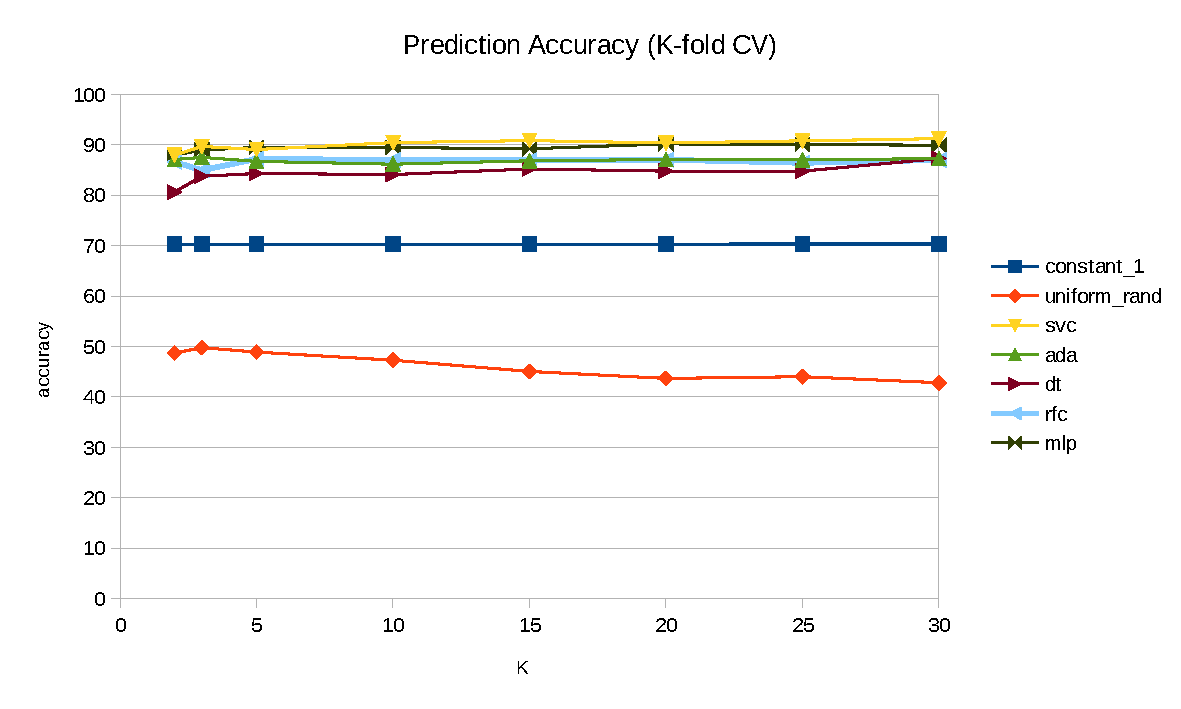
\includegraphics[width=0.5\textwidth]{figures/prediction_accuracy_kfold}
\caption{Prediction accuracy measured using k-fold CV on the whole SNU NPB loop set}
\label{fig:accuracy}
\end{figure}
\begin{comment}
\begin{table}[h!]
    \centering
    \begin{tabular}[c]{|p{1.5cm}|p{1.5cm}|p{1.5cm}|p{1.5cm}|}
        \hline
        ML model & accuracy & recall & precision \\
        \hline
        constant & 70.32 & 100 & 70.32\\
        \hline
        uniform & 46.27 & 41.50 & 69.79\\
        \hline
        SVC & 90.04 & 95.24 & 91.06 \\
        \hline
        AdaBoost & 86.96 & 92.92 & 89.06 \\
        \hline
        DT & 84.36 & 89.57 & 87.90 \\
        \hline
        RFC & 86.65 & 93.22 & 88.47 \\
        \hline
        MLP & 89.40 & 93.77 & 91.39 \\
        \hline
    \end{tabular}
    \caption{Average predictive performance for different ML models measured with a k-fold CV method on the whole set of 1415 SNU NPB loops.}
    \label{tab:average_accuracy}
\end{table}
\end{comment}
\begin{table}
  \begin{minipage}{\columnwidth}
  \begin{center}
    \begin{tabu}{cccc}
      \hline
      \rowfont{\bfseries}
      ML model & accuracy & recall & precision\\\hline
      constant & 70.32 & 100 & 70.32\\
      uniform & 46.27 & 41.50 & 69.79\\
      SVC & 90.04 & 95.24 & 91.06 \\
      AdaBoost & 86.96 & 92.92 & 89.06 \\
      DT & 84.36 & 89.57 & 87.90 \\
      RFC & 86.65 & 93.22 & 88.47 \\
      MLP & 89.40 & 93.77 & 91.39 \\\hline
      \end{tabu}
  \end{center}
  \end{minipage}
  \caption{Average predictive performance for different ML models measured with a K-fold CV method on the whole set of 1415 SNU NPB loops.} 
  \label{tab:average_accuracy}
\end{table}%
\quad Table \ref{tab:average_accuracy} shows the average predictive performance for different ML models. Support Vector Classifier (SVC) model has the highest accuracy and has successfully managed to recall 95,25\% of all parallel loops. Table \ref{tab:icc_stats} shows, that ICC discovers 812 out of 995 parallelisible loops. SVC extends ICC parallelisation capabilities to 945 loops. Despite relatively high precision of 91.06\%, that extension comes at the price of some misprediction errors. Figure \ref{fig:prediction_stats} shows that unsafe (false positive) mispredictions dominate at 65.47\% of cases. Thus we need to devise a scheme, that will protect us and make these errors not that critical.

\begin{figure}[h]
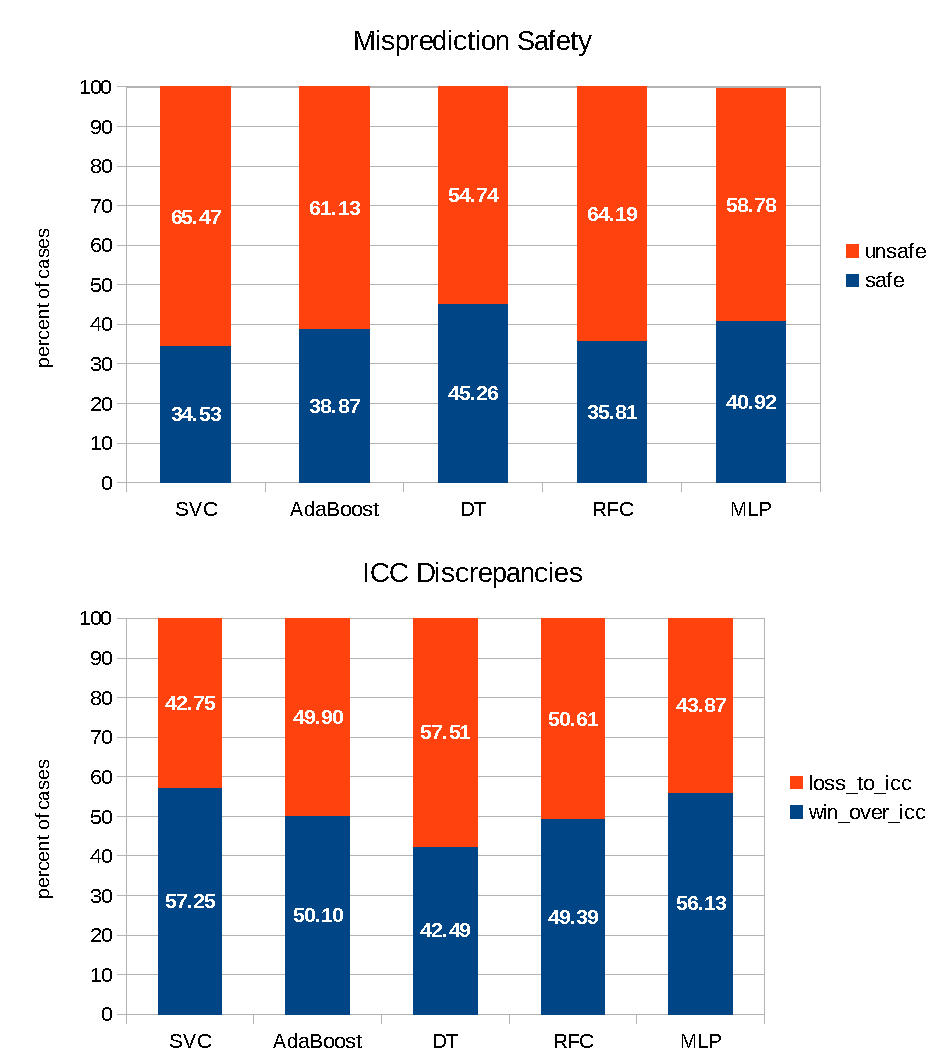
\includegraphics[width=0.5\textwidth]{figures/prediction_stats.pdf}
\caption{Mispredictions nature.}
\label{fig:prediction_stats}
\end{figure}

\subsection{LOOCV SNU NAS Performance}
\label{evaluation_loocv}
\quad While k-fold cross-validation method mixes loops from all 10 SNU NPB benchmarks and provides a good statistical assessment of predictive performance on the whole SNU NPB data set generally, in order to use our predictor with the proposed schemes we need to change our methodology. For that purpose we use modified Leave-One-Out cross-validation (LOOCV) technique. We train our model on 9 benchmarks and test it on the remaining one. Doing so allows us to actually parallelise all correctly predicted parallel loops and get performance numbers for the benchmark being tested.
\begin{comment}
\begin{table*}[t!]
    \centering
    \begin{tabular}[c]{|p{1.5cm}|p{1.0cm}|p{1.5cm}|p{1.3cm}|p{1.0cm}|p{1.5cm}|p{1.3cm}|p{1.0cm}|p{1.5cm}|p{1.3cm}|}
        \hline
        benchmark & \multicolumn{3}{c}{average per model} \vline &	\multicolumn{3}{c}{most frequent} \vline & \multicolumn{3}{c}{uniform} \vline \\
        \hline
	    accuracy & recall &	precision &	accuracy & recall &	precision &	accuracy &	recall	& precision & accuracy \\
	    \hline
        BT & 85.7 & 92.6 & 90.0 & 78.4 & 100.0 & 78.4 & 51.9 & 48.3 & 83.3 \\
        \hline
        CG & 74.2 & 72.4 & 85.7	& 64.4 & 100.0 & 64.4 & 46.7 & 37.9 & 64.7 \\
        \hline
        DC & 72.8 & 71.0 & 51.5	& 29.0 & 100.0 & 29.0 & 55.0 & 37.9 & 28.9 \\
        \hline
        EP & 92.0 &	86.6 & 100.0 & 60.0 & 100.0 & 60.0 & 40.0 & 33.3 & 50.0 \\
        \hline
        FT & 56.5 &	37.9 & 84.4	& 63.0 & 100.0 & 63.0 & 43.5 & 34.5	& 58.8 \\
        \hline
        IS & 74.0 &	97.5 & 61.3	& 40.0 & 100.0 & 40.0 &	45.0 & 37.5	& 33.3 \\
        \hline
        LU & 90.1 &	90.7 & 96.3	& 78.0 & 100.0 & 78.0 & 46.1 & 45.0	& 76.1 \\
        \hline
        MG & 64.9 &	87.6 & 57.8	& 45.7 & 100.0 & 45.7 &	43.2 & 32.4	& 36.4 \\
        \hline
        SP & 88.8 &	94.7 & 92.2	& 83.4 & 100.0 & 83.4 &	46.6 & 46.4	& 81.7 \\
        \hline
        UA & 75.9 &	83.8 & 83.9	& 72.9 & 100.0 & 72.9 &	48.4 & 47.2	& 72.5 \\
        \hline
    \end{tabular}
    \caption{Predictive performance on different for different ML models measured with a k-fold CV method on the whole set of 1415 SNU NPB loops.}
    \label{tab:average_accuracy}
\end{table*}
\end{comment}

\begin{table*}
  \begin{minipage}{\textwidth}
  \begin{center}
    \begin{tabu}{c|ccc|ccc|ccc}
      \hline
      \rowfont{\bfseries}
      Benchmark & \multicolumn{3}{c}{Average Per Model} \vline & \multicolumn{3}{c}{Most Frequent} \vline & \multicolumn{3}{c}{Uniform}\\\hline
      \rowfont{\bfseries}
      Accuracy & Recall & Precision & Accuracy & Recall & Precision & Accuracy & Recall	& Precision & Accuracy\\\hline
      BT & 85.7 & 92.6 & 90.0 & 78.4 & 100.0 & 78.4 & 51.9 & 48.3 & 83.3 \\
      CG & 74.2 & 72.4 & 85.7	& 64.4 & 100.0 & 64.4 & 46.7 & 37.9 & 64.7 \\
      DC & 72.8 & 71.0 & 51.5	& 29.0 & 100.0 & 29.0 & 55.0 & 37.9 & 28.9 \\
      EP & 92.0 &	86.6 & 100.0 & 60.0 & 100.0 & 60.0 & 40.0 & 33.3 & 50.0 \\
      FT & 56.5 &	37.9 & 84.4	& 63.0 & 100.0 & 63.0 & 43.5 & 34.5	& 58.8 \\
      IS & 74.0 &	97.5 & 61.3	& 40.0 & 100.0 & 40.0 &	45.0 & 37.5	& 33.3 \\
      LU & 90.1 &	90.7 & 96.3	& 78.0 & 100.0 & 78.0 & 46.1 & 45.0	& 76.1 \\
      MG & 64.9 &	87.6 & 57.8	& 45.7 & 100.0 & 45.7 &	43.2 & 32.4	& 36.4 \\
      SP & 88.8 &	94.7 & 92.2	& 83.4 & 100.0 & 83.4 &	46.6 & 46.4	& 81.7 \\
      UA & 75.9 &	83.8 & 83.9	& 72.9 & 100.0 & 72.9 &	48.4 & 47.2	& 72.5 \\\hline
      \end{tabu}
  \end{center}
  \end{minipage}
  \caption{Average predictive performance for different ML models measured with a K-fold CV method on the whole set of 1415 SNU NPB loops.} 
  \label{tab:average_accuracy}
\end{table*}%


\begin{figure}[h]
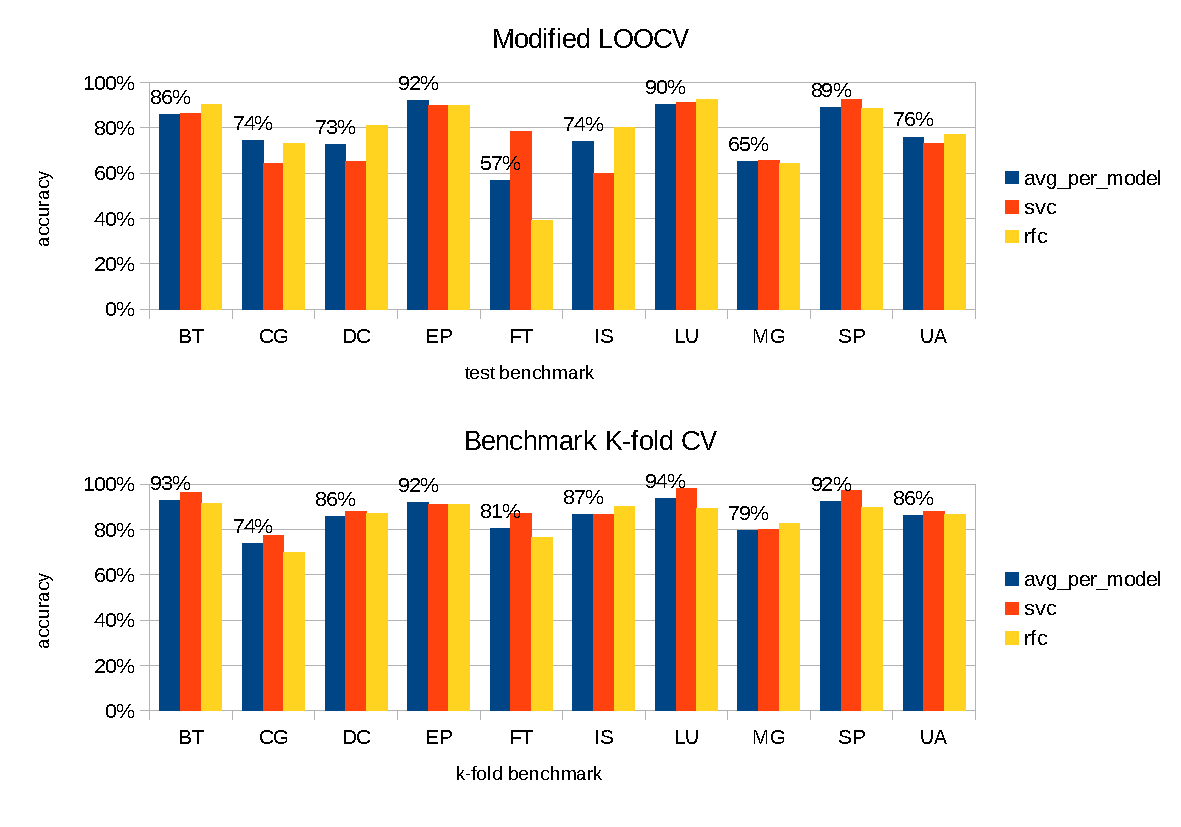
\includegraphics[width=0.5\textwidth]{figures/LOOCV_accuracy.pdf}
\caption{Prediction accuracy measured using k-fold CV on the whole SNU NPB loop set}
\label{fig:accuracy}
\end{figure}

\section{Parallelization Assistant}
\label{practical_applications}
\quad Achieving high predictive performance is not enough. We need to find a real practical application of our loop parallelizability predictor. Due to statistical nature inherent to all machine learning techniques it is impossible to eliminate all prediction errors completely. While false negative mispredictions might just miss available parallelization opportunities and lose some performance, false positive mispredictions can break the program and are the most critical in the context of our ML problem.\newline\null
\quad Taking the above mentioned fact into the consideration we propose to integrate our trained predictor into an assistant scheme, which leaves the final parallelization decision up to a programmer. Taking application profile as an input our assistant computes a ranking score for every loop in the application. The ranking score is defined as the product of loop running time (actually, the fraction of the whole application running time this loop takes to run) and the shifted sigmoid function of the probability that the loop is parallelizable. The latter is extracted out of the trained ML model. The figure \ref{fig:sigmoid_3d} plots the function.
\begin{figure}[h]
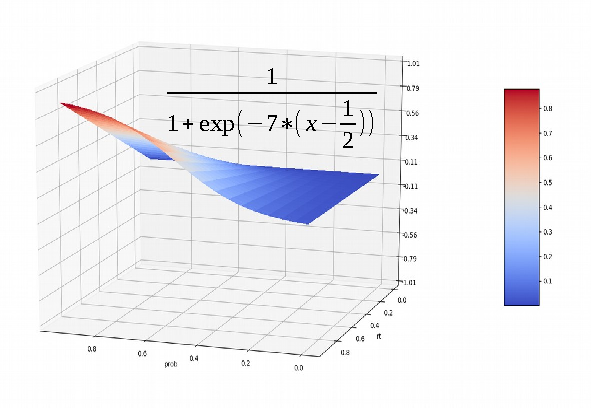
\includegraphics[width=0.5\textwidth]{figures/sigmoid_3d.pdf}
\caption{Filter function used in our assistant. We used a slightly modified for our purposes version of a well known sigmoid (logistic) function.}
\label{fig:sigmoid_3d}
\end{figure}
With a more detailed examination it is visible, that the shape of the function is chosen in a way, that it ranks parallelizable long-running program loops the highest and tries to amplify all non-parallelizable loops down. Even the longest running non-parallelizable program loops are going to rank lower than parallelizable loops with a more or less noticeable running time. The effect is better demonstrated with the case study presented on the figure \ref{fig:ft_loop_ranking}, which highlights the contrast between different rankings of FT benchmark loops. 
\begin{figure*}[!h]
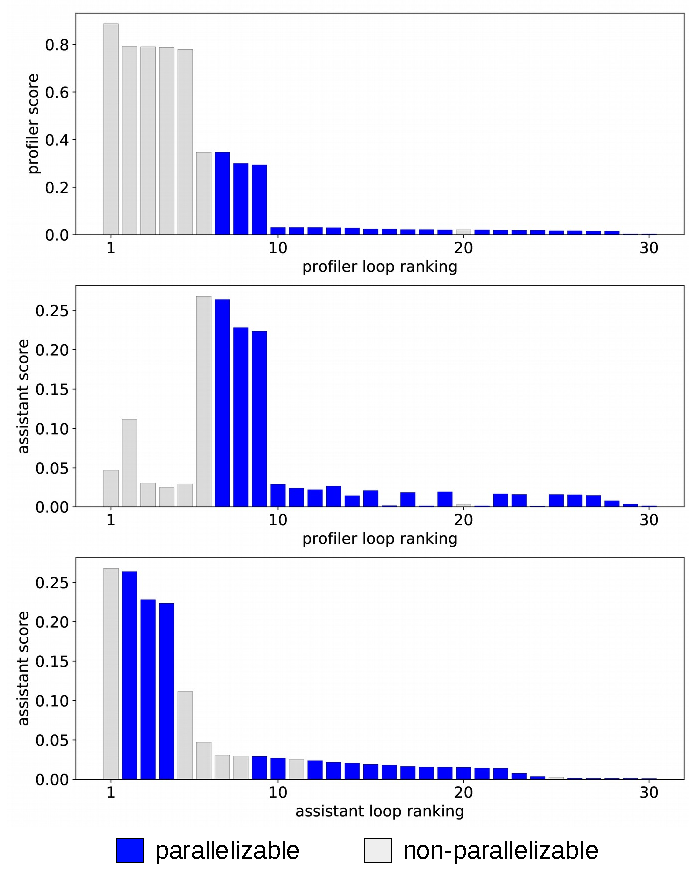
\includegraphics[width=\textwidth]{figures/ft_filter.pdf}
\caption{Loop ranking reordering for the 46 loops of SNU NPB FT benchmark. The top and bottom plots on the left show the change in the relative heights of loop bars, taking place with a switch from runtime to product scoring function. The two plots on the right compare the final rankings and show, that black non-parallelisable loops ended up being moved towards the back of the list, whereas white and grey parallelizable loops moved towards the front.}
\label{fig:ft_loop_ranking}
\end{figure*}
Top left and right pictures are identical and rank benchmark loops according to the running time fraction loops constitute. The problem with the pure runtime fraction order is that it ranks long-running program loops the highest independent of their parallelizability. If a programmer starts to paralleliza application following the runtime based order, he is going to waste his time and efforts on the loops one cannot parallelize anyway. The left and right plots at the bottom of the figure demonstrate a transformation in the loop ranking our assistant does. Vertical axes of these plots correspond to the values our shifted sigmoid ranking function (see figure \ref{fig:sigmoid_3d}) takes. The bottom left plot shows how the relative height of the bars changes with a switch from a loop runtime to our scoring function. The bottom right picture shows that such a change actually moves true parallel loops toward the beginning of the list. The longer loop takes to run, the bigger the move. On the other hand non-parallelizable loops move towards the back of the list (almost independent of their running time). The improved ranking of FT loops allows a programmer to immediately start benchmark parallelisation with the most important loops and don't waste time looking at long-running loops, which cannot be parallelized by their nature anyway.\newline\null
\begin{figure}[h]
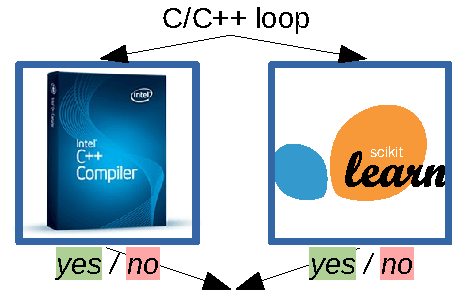
\includegraphics[width=0.5\textwidth]{figures/icc_competition_scheme.pdf}
\caption{First predictor application. Smart parallelisation adviser. }
\label{fig:icc_competition_scheme}
\end{figure}
\quad There is another important property implicitly living in our assistant. In its static analysis Intel \cpp{} Compiler has to be conservative and misses some parallelization opportunities: if it cannot prove that there are no parallelization prohibiting dependencies in the loop, then we cannot parallelize it, even if the loop is actually parallelizable.
\begin{comment}
\begin{table}[h]
    \centering
    \begin{tabular}[c]{|p{1.0cm}|p{1.5cm}|p{1.5cm}|p{2cm}|}
        \hline
        ICC & predictor & true parallel & classification bucket \\
        \hline
        0 & 0 & 0 & correct 0 (no) prediction \\
        \hline
        0 & 0 & 1 & missed opportunity \\
        \hline
        0 & 1 & 0 & false positive \\
        \hline
        0 & 1 & 1 & discovery \\        
        \hline
        1 & 0 & 0 & impossible \\
        \hline
        1 & 0 & 1 & icc shielding \\
        \hline
        1 & 1 & 0 & impossible \\
        \hline
        1 & 1 & 1 & correct 1 (yes) prediction \\  
        \hline
    \end{tabular}
    \caption{All the possible ICC competition scheme combinations}
    \label{tab:combinations_table}
\end{table}
\end{comment}
\begin{table}
  \begin{minipage}{\columnwidth}
  \begin{center}
    \begin{tabu}{M{0.5cm}M{1.2cm}M{2.0cm}M{3.5cm}}
      \hline
      \rowfont{\bfseries}
      ICC & Predictor & True Parallel & Classification Bucket\\%\hline
      \hline
      0 & 0 & 0 & correct 0 (no) prediction\\
      0 & 0 & 1 & missed opportunity\\
      0 & 1 & 0 & false positive\\
      0 & 1 & 1 & discovery\\
      1 & 0 & 0 & impossible\\
      1 & 0 & 1 & icc shielding\\
      1 & 1 & 0 & impossible\\
      1 & 1 & 1 & correct 1 (yes) prediction\\\hline  
    \end{tabu}
  \end{center}
  \end{minipage}
  \caption{All the possible ICC competition scheme combinations.}
  \label{tab:combinations_table}
\end{table}%
Having learnt loop parallelizability property better than ICC, our ML model can predict those loops as parallelizable, thus extending ICC parallelizm discovery capabilities. The visible effect of this is that our assistant gives high parallelizability probabilities to those loops and thus moves them toward the beginning of the ranking, despite the fact that ICC refused to parallelize them at all. We name such cases as "discovery".\newline\null
\quad To better illustrate the property described above we conduct the following experiment. We put our predictor in the same harness with the ICC and assign the former a supplementary role to perform.\newline\null
\quad Figure \ref{fig:icc_competition_scheme} demonstrates the setting of the experiment. The two components (ICC and predictor) independently classify loops as parallelizable or not. There are a total of 6 possible classification outcomes our schem might potentially produce. Table \ref{tab:combinations_table} summarizes them. The most interesting cases here are the cases, when predictor disagrees with ICC. If predictor says "yes, parallelisible" and ICC compiler says the opposite we might either discover a new parallelisation opportunity (case 011), or make a critical false positive mispredicton (case 010). In the 101 case ICC compiler "shields" ML predictor from making a false negative misprediction and losing performance. When feedback components agree with each other we do not gain anything over single ICC scheme. They might both say "no" to a truly parallelisible loop and thus miss some opportunities.  

\begin{comment}
As we show in the section \ref{evaluation}, it increases the amount of parallelism discovered in a program. Discovered parallelism does not necessarily materialises into real performance gains. To accelerate a program parallelisable loop has to be profitable. To take loop profitability into account we propose a second scheme, which takes the profile of a program and produces a loop ranking. This ranking is better than just a mere profile-based loop running time order in that it filters non-parallel loops out and moves them to the back of the ranking.

Moreover, to be useful our schemes do not even require a close to perfect predictor accuracy.

Ideal loop ranking would put all parallelilasible loops at the front and order them by their running time. 

As we can see from the plot, our function amplifies probabilities above 50\% and diminishes probabilities below $\frac{1}{2}$ line. At the same time low probabilities are still non zero. Such function shape protects us from filtering long running false negatives out of the ranking.

\end{comment}

%\quad In these scheme we propose a machine learning based tool, which can be used to speed the process of software parallelisation by pointing out the "right" loops for a programmer to direct his/her efforts. The tool takes several inputs. First input is the configuration of ML pipeline to use (ML model, ML feature selection techniques, etc.). Second, we need a set of programs, which can be used to train our ML model to recognise parallelisable loops. In our training scheme we propose to use static program features only (although dynamic features can be added as well). Such a scheme captures static properties (dependencies, sizes, instructions, etc.) of loops and thus their algorithmic parallelisability, but does not take into consideration the actual profitability of parallelisation of such loops. A loop can be parallelisible, but a lightweight one, without consuming much a a program running time. Not only the parallelisation of such loops seems meaningless, but can even slow the program down. To deal with that problem our tool takes the profile of the application the tool is used on. takes a set of programs for a training of ML model.

\subsection{ICC competition scheme}
\label{evaluation_icc_competition}
\quad The first ML model practical use scenario is outlined in the section \ref{application_icc_competition}. In that scenario we harness ML model together with ICC compiler and provide a programmer with a feedback regarding loop parallelisability using outputs of both components. As our model has been trained with expert OpenMP labels along with regular ICC reports, it can potentially extend ICC capabilities in the loop parallelism discovery.\newline\null
\quad Before we ran that experiment we conducted a research into SNU NPB source code base and its parallelisation with ICC compiler. We identified all cases, where ICC misses parallel loops and classified the reasons into separate buckets. Table \ref{tab:icc_missed_opportunities} shows the results.

\begin{table}[h!]
    \centering
    \begin{tabular}[c]{|p{2cm}|p{2cm}|p{2cm}|}
        \hline
        unrecognised reduction & array privatization & AA conservativeness \\
        \hline
        18 & 7 & 60 \\
        \hline
        unknown iteration number & static dependencies & too complex \\
        \hline
        7 & 46 & 22 \\
        \hline
        uninlined calls & other & total \\
        \hline
        4 & 4 & 168   \\
        \hline
    \end{tabular}
    \caption{Classification of loops missed by Intel Compiler for various reasons}
    \label{tab:icc_missed_opportunities}
\end{table}

After the study of ICC limitations on SNU NPB benchmarks we set the experiment to assess the performance of our scheme in the following way. We repeatedly ran k-fold CV on the whole set of SNU NPB loops and clustered them all into separate buckets according to the following combinations table .

Figure \ref{fig:icc_competition} shows the final distribution of all the cases as percentages of the total number of experiments for different ML models. As it can be seen from the figure in majority of cases our ML based tool agrees with ICC and either classifies truly non-parallel loops as non-parallel and truly parallel as parallel. We can explain this by the fact, that we trained our ML model with ICC optimization reports and to some degree our tool learnt ICC reasonings. However, sometimes there are disagreements between ICC and our tool. We can classify these disagreements into 3 buckets: the one, where our predictor makes a critical mistake by prediction non-parallel loop to be parallelisible; the one, where our predictor discovers a parallell loop missed by ICC.       

\begin{figure*}[t!]
\centering
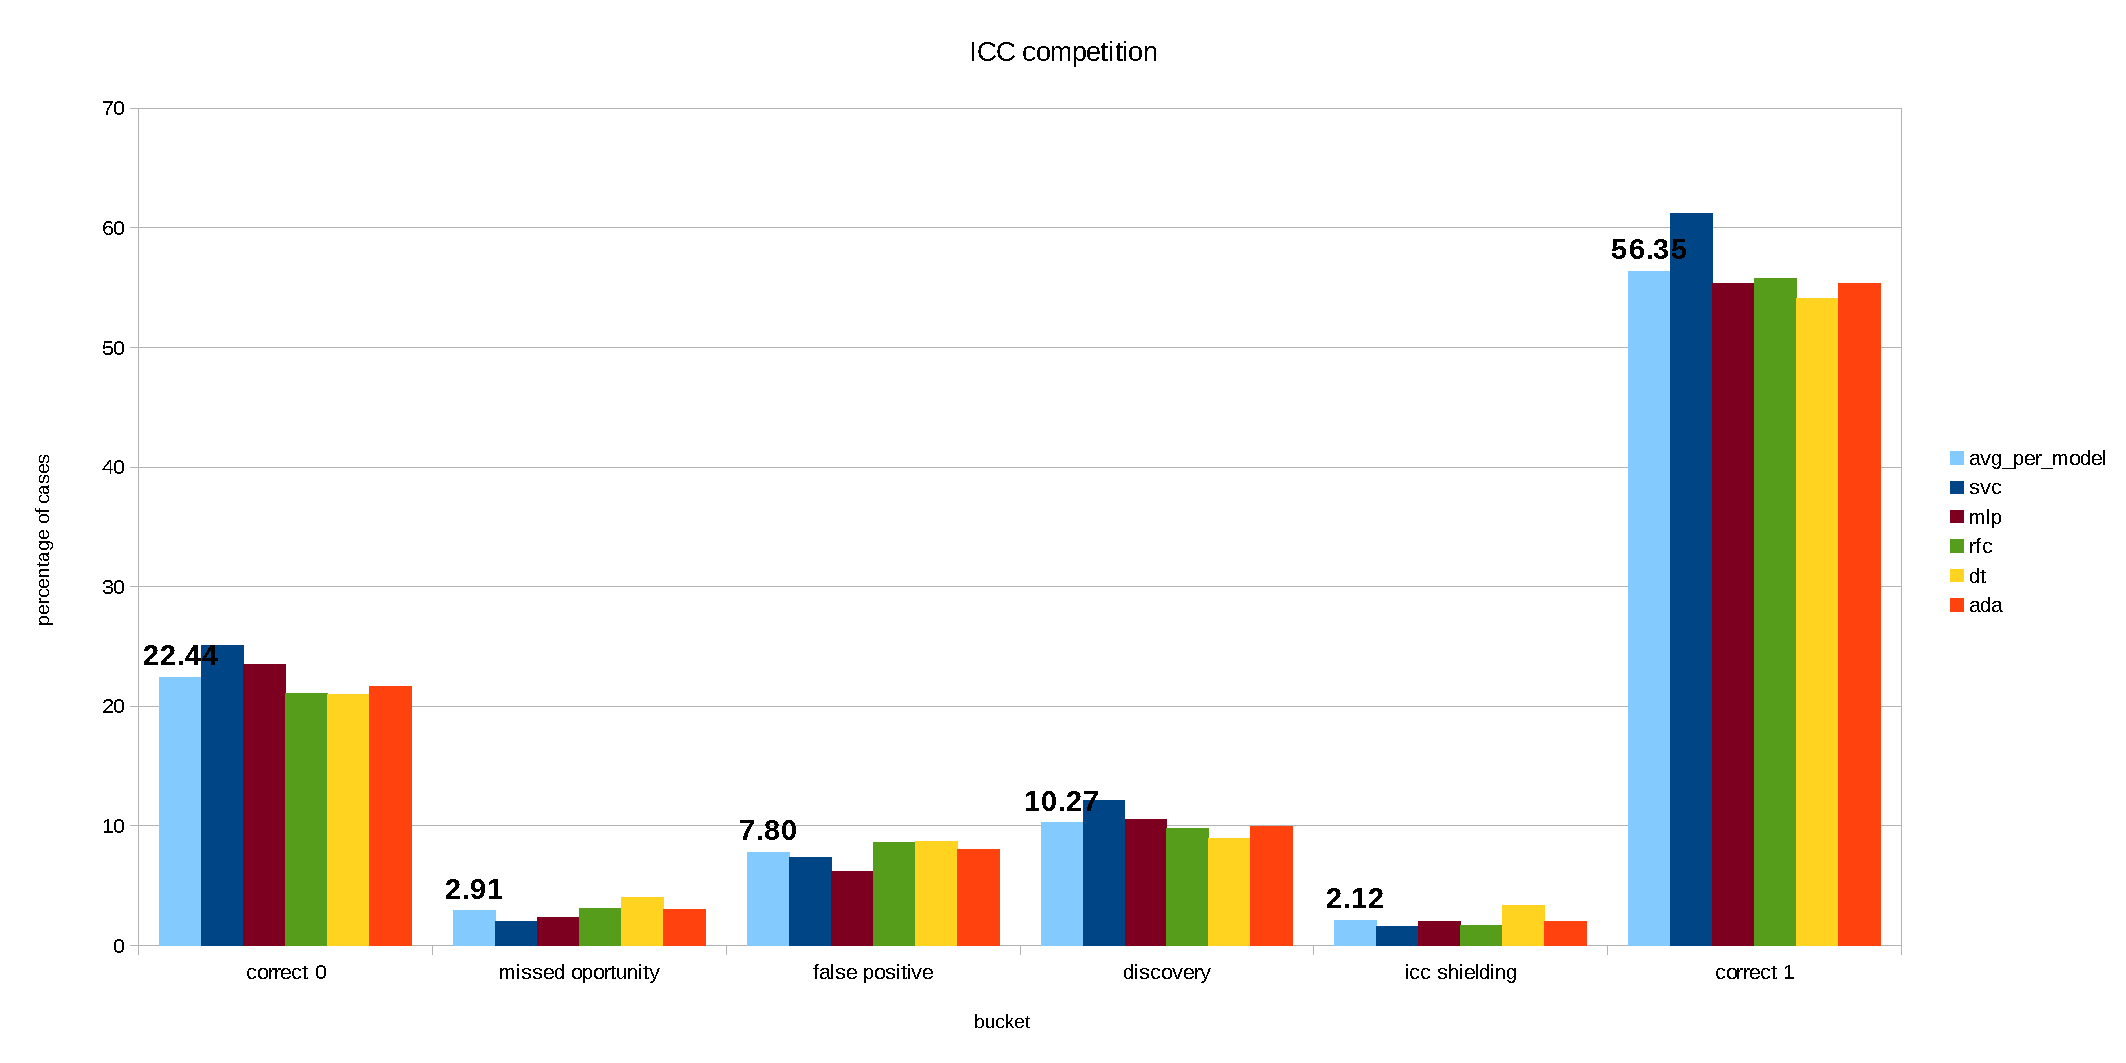
\includegraphics[width=\textwidth]{figures/icc_competition.pdf}
\caption{Prediction accuracy measured using k-fold CV on the whole SNU NPB loop set}
\label{fig:icc_competition}
\end{figure*}

\section{Assistant Deployment on SNU NPB}
\label{evaluation}
\quad Section [] describes the internal workings of our devised software parallelisation assistant and shows how the latter extends the parallelism discovery capability of Intel Compiler. In this section we are actually demonstrating the deployment of our assistant on SNU NAS Parallel Benchmarks.    
\begin{comment}
\quad Program running time on a real system is the most important characteristic, as far as software parallelisation is concerned. Thus, at the end of a day we aim to assess our techniques with running time used as the major criterion. In this section we also provide all reports on the predictive performance of our models, assessed by the means of K-fold CV and modified LOOCV techniques (see sections \ref{evaluation_kfold} and \ref{evaluation_loocv}). Section \ref{evaluation_icc_competition} reports on our ICC competition scheme (see section \ref{application_icc_competition}). At the end we show, that our smart assistant (see \ref{application_profile_filter}) can improve a straightforward profile based parallelisation and converge to performance levels of the best parallel version faster (see section ).
\quad This section reports on the assessment of software parallelisation assistant scheme proposed in the section \ref{application_profile_filter} of the paper. As the major fraction of program execution time is spent in program loops, they represent the most important program structure one should aim to parallelise. The ultimate goal of our \textit{smart} software parallelisation assistant is to ease the manual software parallelisation process by pointing out the program loops, where a programmer should concentrate his efforts. Following the order provided by our assistant a programmer should approach the best achievable performance levels faster then he would by following a profile-based loop order.\newline\null
\end{comment}
\quad But before we can assess our assistant we need to conduct a study of performance we could potentially extract from SNU NPB benchmarks. To explore the potential present in SNU NPB benchmarks we measured the running times of differently compiled versions. Figure \ref{fig:snu_npb_performance} shows the results. It can be seen, that ICC compiler not only fails to achieve noticeable speedups, but actually significantly slows performance down on some of the benchmarks. While BT, CG, EP, FT, IS benchmarks show a good speedup for a manually parallelised benchmark developer version, the rest do not exhibit significant speedups with UA benchmark showing even a slowdown.\newline\null
\quad Our \textit{smart} parallelisation adviser reorders a runtime ordered list of benchmark loops in a way it thinks that minimises programmer parallelisation efforts and helps to close performance gap between a serial version and a parallel one. Our technique is not applicable to DC and IS benchmarks: these benchmarks get their parallel speedups from OpenMP parallel sections and not from parallel loops. Parallelisation of loops in these benchmarks (be it profile ordered list or the one of our smart adviser) actually slows them down. Figure \ref{fig:performance_convergence_line} shows performance convergence curves for the most interesting benchmarks.
\quad In order to deploy our adviser on SNU NPB benchmarks we have to use modified LOOCV methodology. We take the test benchmark and train our adviser on the 9 remaining ones. As section \label{loocv_accuracy} shows such a methodology has a lower predictive performance due to training set incompleteness, which potentially limits the success of our technique.   
\begin{figure*}[t!]
\centering
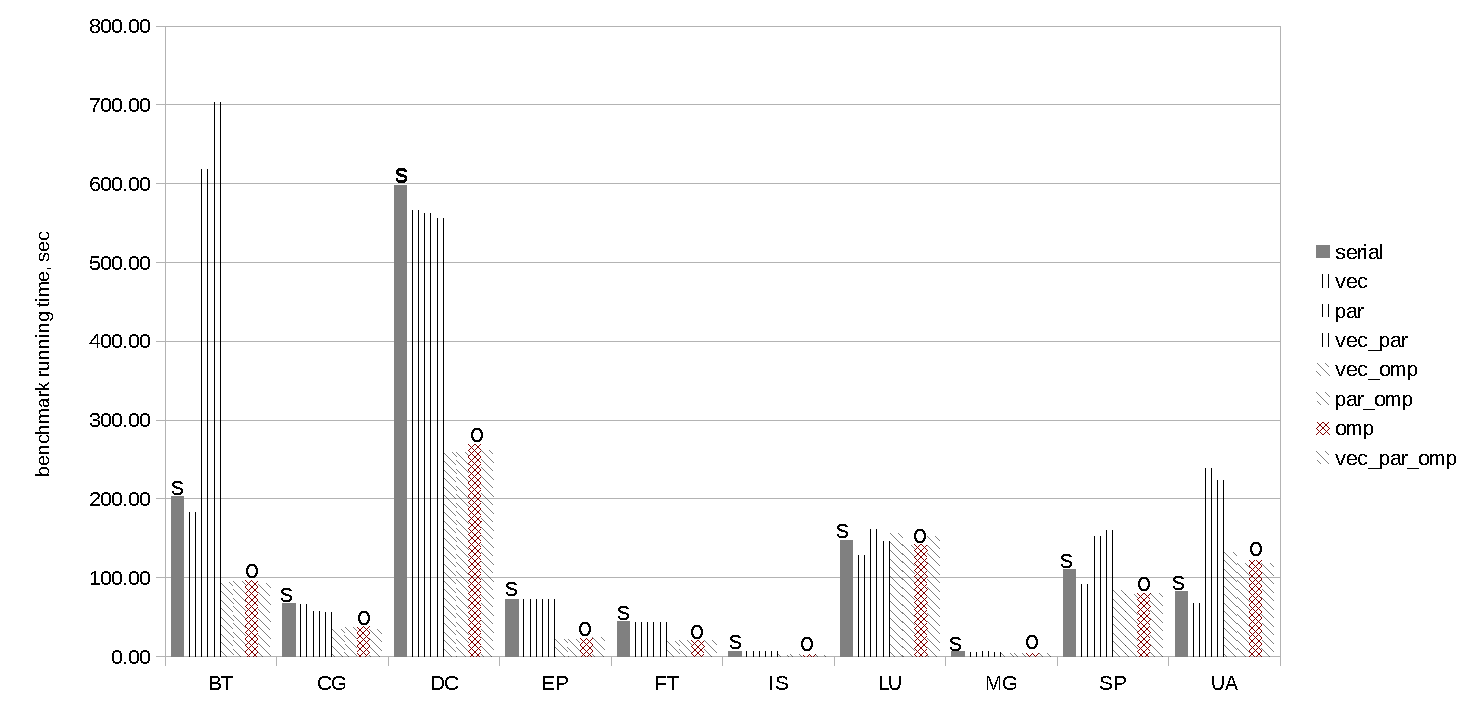
\includegraphics[width=\textwidth]{figures/benchmark_runtime.pdf}
\caption{SNU NPB running times for different compilation options: serial, automatic parallelisation and vectorization, OpenMP benchmark expert developer version and all the possible combinations of those.}
\label{fig:snu_npb_performance}
\end{figure*}
\begin{figure*}[t!]
\centering
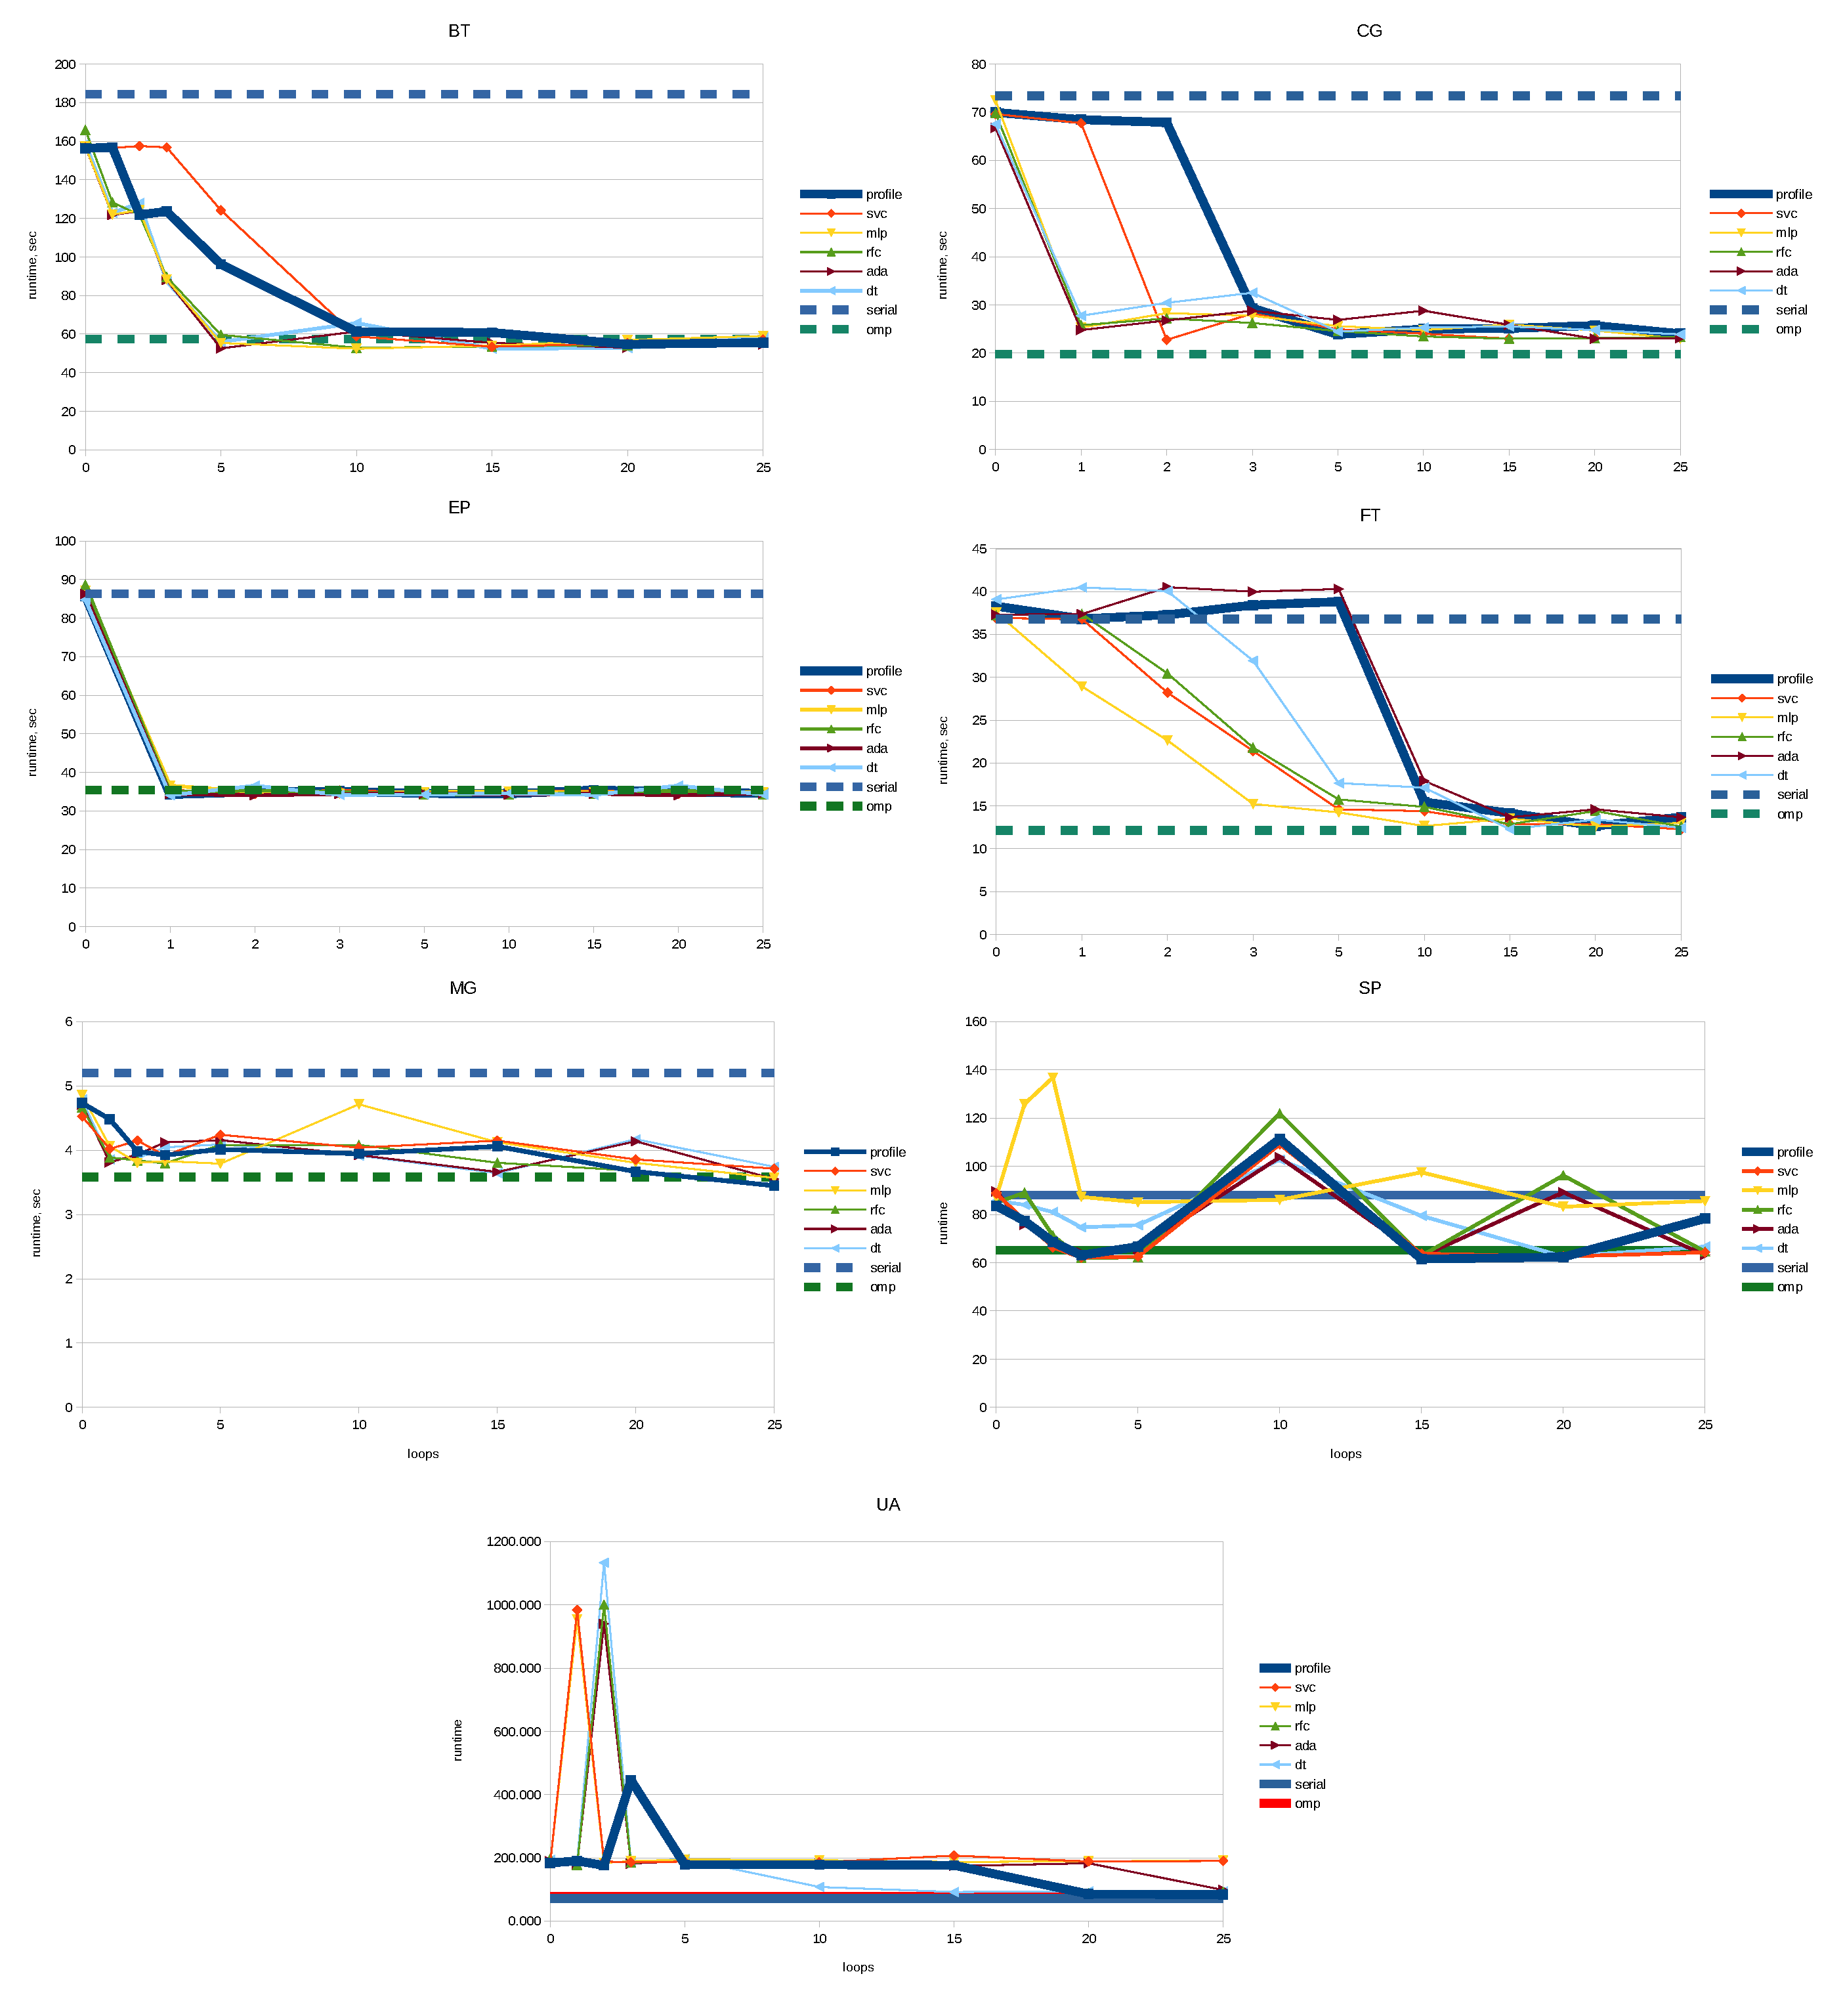
\includegraphics[width=\textwidth]{figures/perf_conv_curves.pdf}
\caption{Example of performance convergence curves for the most representativ eBT, CG, FT, UA benchmarks. Our technique outperforms a simple profile based loop ranking for BT, CG and FT, but  }
\label{fig:performance_convergence_line}
\end{figure*}
\begin{comment}
\quad The common general thing about all SNU NAS benchmarks we observed is that the main portion of benchmark speedup comes from a coarse-grain manual parallelisation done by its developers. The main loops preceded by OpenMP pragmas are quite big and complex. Usually they contain calls to different functions, which do not always get inlined, as well as a lot of multidimensional arrays with complex index computations. Many array references happen indirectly and thus require runtime behaviour knowledge for their analysis. Parallelisation of such loops requires a thorough comprehension of the source code by a programmer, and is beyond the capabilities of the state-of-the-art automatic tools.\newline
\quad Intel compiler vectorises and parallelises quite a significant number of SNU NAS benchmark loops, but these loops are not the main ones. When we measure the performance of parallel and vector codes generated by Intel compiler, we observe running times being slightly better than in serial versions for vector codes and significant slowdowns for automatic ICC parallelisation.       
\quad The major weakness of Intel compiler, as well as our trained loop parallelisability classifier is that they mostly discover relatively fine-grain parallelism and miss opportunities seized by manual coarse-grain parallelisation. SNU NAS benchmarks contain a lot of big loops with deep nesting and uninlined function calls inside. SNU NAS developers have deep benchmark behaviour understanding and know exactly where even such loops can be parallelised, but that knowledge is far beyond the sight of automatic tools. 
\quad Parallelism present in EP and DC benchmarks is undetectable neither by Intel compiler nor by our oracle. DC benchmark contains only 1 parallel section encapsulating many function calls and complex control flow. Such parallelism cannot be detected in principle. Performance of EP benchmark depends heavily on the single loop with a reduction. SNU NPB developers have successfully manually parallelised this loop, but neither ICC nor trained oracle could find parallelism in it. Oracle predicted thsi loop to be 40\% parallelisible. The loop is complex and contains 2 inner loops, where reduction variables are buried as well as timer and random generator function calls.\newline
\quad Our scheme does not utilise all the coarse-grain parallelism of FT benchmark as well. Developers parallelise outermost loops of loop nests, whereas our classifier finds parallelism only in a modestly-sized inner loops, which do not contain function calls (thus operating at a finer level). Such finer parallelisation is not always beneficial and introduces overheads from implicit OpenMP barriers.
\quad Our scheme advised us to parallelise almost all BT benchmark loops, which contain OpenMP pragma in the original hand-parallelised benchmark version. There are a couple of missed OpenMP pragmas. Moreover, our scheme advises us to parallelise inner loops with a finer grains of parallelism, but doing so results in a slowdown, rather than speedup. So we take predictor's feedback and apply it on the top of our common sense that only outer loops should be parallelised to avoid synchronisation overheads and stalls.    
\end{comment}
\quad Table illustrates the final SNU NPB parallelisation report.
\begin{table*}[h!]
    \centering
    \begin{tabular}[c]{|p{1cm}|p{1cm}|p{1cm}|p{1cm}|p{1cm}|p{1cm}|p{1cm}|p{1cm}|p{1cm}|p{1cm}|p{1cm}|p{1cm}|}
        \hline
        \multirow{2}{2.5cm}{benchmark} & \multicolumn{3}{c}{benchmark running time, sec} \vline & \multicolumn{2}{c}{speedup, times} \vline & \multicolumn{6}{c}{loops number} \vline\\\cline{2-12}
        & serial & openmp & critical & openmp speedup & critical speedup & profile & svc & mlp & rfc & ada & dt\\\cline{1-12}
        \hline
        BT & 158.76 & 57.36 & 56.57 & 2.77 & 2.81 & 6 & \cellcolor[HTML]{FA8D8D} 8 & \cellcolor[HTML]{7BB66B} 4 & \cellcolor[HTML]{7BB66B} 5 & \cellcolor[HTML]{7BB66B} 3 & \cellcolor[HTML]{7BB66B} 5\\
        \hline
        CG & 69.38 & 19.77 & 25.06 & 3.51 & 2.77 & 3 & \cellcolor[HTML]{7BB66B} 2 & \cellcolor[HTML]{7BB66B} 1 & \cellcolor[HTML]{7BB66B} 1 & \cellcolor[HTML]{7BB66B} 1 & \cellcolor[HTML]{7BB66B} 1\\
        \hline
        DC & 698.82 & 254.29 & 698.82 & 2.75 & 1.00 & 0 & \cellcolor[HTML]{91A1FA} inf & \cellcolor[HTML]{91A1FA} inf & \cellcolor[HTML]{91A1FA} inf & \cellcolor[HTML]{91A1FA} inf & \cellcolor[HTML]{91A1FA} inf\\
        \hline
        EP & 86.35 & 35.40 & 35.07 & 2.44 & 2.46 & 1 & \cellcolor[HTML]{91A1FA} 1 & \cellcolor[HTML]{91A1FA} 1 & \cellcolor[HTML]{91A1FA} 1 & \cellcolor[HTML]{91A1FA} 1 & \cellcolor[HTML]{91A1FA} 1\\
        \hline
        FT & 36.81 & 12.13 & 14.69 & 3.03 & 2.51 & 9 & \cellcolor[HTML]{7BB66B} 4 & \cellcolor[HTML]{7BB66B} 3 & \cellcolor[HTML]{7BB66B} 4 & \cellcolor[HTML]{91A1FA} 9 & \cellcolor[HTML]{7BB66B} 5\\
        \hline
        IS & 4.75 & 1.35 & 4.63 & 3.53 & 1.03 & inf & \cellcolor[HTML]{91A1FA} inf & \cellcolor[HTML]{91A1FA} inf & \cellcolor[HTML]{91A1FA} inf & \cellcolor[HTML]{91A1FA} inf & \cellcolor[HTML]{91A1FA} inf\\
        \hline
        LU & 115.46 & 55.00 & 140.53 & 2.10 & 0.82 & inf & \cellcolor[HTML]{91A1FA} inf & \cellcolor[HTML]{91A1FA} inf & \cellcolor[HTML]{91A1FA} inf & \cellcolor[HTML]{91A1FA} inf & \cellcolor[HTML]{91A1FA} inf\\
        \hline
        MG & 5.20 & 3.58 & 3.94 & 1.45 & 1.32 & 3 & \cellcolor[HTML]{91A1FA} 3 & \cellcolor[HTML]{91A1FA} 3 & \cellcolor[HTML]{91A1FA} 3 & \cellcolor[HTML]{91A1FA} 3 & \cellcolor[HTML]{91A1FA} 3\\
        \hline
        SP & 86.65 & 65.19 & 62.90 & 1.33 & 1.38 & 3 & \cellcolor[HTML]{91A1FA} 3 & \cellcolor[HTML]{FA8D8D} inf & \cellcolor[HTML]{91A1FA} 3 & \cellcolor[HTML]{91A1FA} 3 & \cellcolor[HTML]{FA8D8D} 20\\
        \hline
        UA & 71.82 & 78.56 & 189.66 & 0.91 & 0.38 & 19 & \cellcolor[HTML]{FA8D8D} 30 & \cellcolor[HTML]{FA8D8D} 30 & \cellcolor[HTML]{91A1FA} 19 & \cellcolor[HTML]{FA8D8D} 22 & \cellcolor[HTML]{7BB66B} 10\\
        \hline
    \end{tabular}
    \caption{Final SNU NPB manual paralelization report. Running times and corresponding speedups are provided for \textit{serial}, \textit{OpenMP} and \textit{critical loops only} benchmark versions. OpenMP is the hand-parallelized version of SNU NPB developers. Critical  }
    \label{tab:final_parallel_table}
\end{table*}

\section{Related Work}
\label{related_work}

\subsection{Loop Parallelisation}

\subsection{Machine Learning in Compilers}
\quad Correctness is critical

it can be used for topics ranging from selecting the best compiler flags to determining how to map parallelism to processors.

tradition in computer science in increasing automation

It also brings compilation nearer to the standards of evidence based science.

It introduces an experimental methodology where we separate out evaluation from design and considers the robustness of solutions.

Next, in Section V, we review how previous work chooses quantifiable properties, or features, to represent programs.

\subsection{Machine Learning and Parallelisation}

Machine learning techniques have already been applied in the field of compilers, but their application is mostly concentrated in the task of auto-tuning and optimal mapping of software onto a range of diverse hardware platforms. That fact has a reasonable explanaition. Compiler has to produce semantically correct translation of high-level source program into the instructions of a target machine. Statistical nature of machine learning approaches and their inherent errors limit their application in the field of compilers. Machine learning approaches has been applied to the tasks of selecting the best compiler flags for mapping software onto different kinds of hardware. This areas are safe for machine learning application. 

In this work on the contrary we step into potentially dangerous machine learning application area. We investigate the task of loop parallelisability prediction. We calculate the number of unsafe error cases and propose a scheme ensuring the final correctness of produced parallel software.

This is not the only effort of extracting the best performance out of software potentially compromising its correctness. There is a vast body of research of supplementing compiler static analyses with dynamic information. These techniques have a property that they cannot generally prove correctness of profile-guided transformations for the whole range of possible program inputs.

Work \cite{fried_ea:2013:icmla} is similar to ours, but it has a number of differences.  

\section{Summary \& Conclusions}

The ultimate goal of this work has always been to provide a programmer with a feedback on the parallelisability of software in general and loops in particular. The work has evolved from parallelisability correlations of single metrics (features) to a machine learning based tool for filtering runtime program profile and providing the resulting loop ranking for a programmer.\newline\null
\quad The ultimate performance of the tool depends on many factors. First 

\subsection{Future Work}

Having received some motivating results, there are still certain areas of improvement. The tool consists of a number of co-designed parts. Their tuning for maximum overall performance can be done infinitely. The ultimate performance of the tool is affected by a number of factors. The main factor is the nature of the programs (benchmarks) being used for ML training and testing stages. SNU NAS benchmarks are quite diverse in terms of the loops they contain. Loops have different sizes, nesting structures, parallelism patterns.

\quad We believe, that our idea can be worked on and improved even further. There are several possible potential steps.

\quad Our scheme consists of a number of components and steps. First we select training and testing programs, then we engineer the set of representative ML features. After 

\quad First, SNU NPB benchmarks have certain features and properties that reveal themselves in our work. 
\quad In our work we use SNU NAS Parallel Benchmarks for assessment of our machine learning based technique. Majority of SNU NPB benchmarks concentrate their running time in a relatively small set of critical loops. That fact presents a problem for a full scale assessment of our technique.      



Our tool consists of a lot of components to be tuned. The tuning work can be done infinetely in the attempt to get the best possible performance on a wider range of programs and benchmarks.    

\subsection{Future Work}

\section{SPLASH Conference}

Systems, Programming, Languages, and Applications: Software for Humanity (SPLASH).
Software Engineering for Parallel Systems (SEPS).

\bibliographystyle{ACM-Reference-Format}
\bibliography{main}

%\printbibliography

\end{document}
